\section{Experiments Results}\label{body_experiments_results}
\paragraph{Motivation}\label{exp_results_motivation}
The primary motivation for investigating multi-generator GAN architectures for Generative Data Augmentation (GDA) stems from a suggestion by Ian Goodfellow on the Lex Fridman Podcast \cite{fridman2019Goodfellow}. He proposed leveraging the diversity inherent in multiple generative models trained on the same data to potentially improve downstream classifiers:

\begin{quotation}
    \noindent So one thing I think is worth trying [\dots] is, what if you trained a whole lot of different generative models on the same training set, create samples from all of them and then train a classifier on that. Because each of the generative models might generalize in a slightly different way, they might capture different axes of variation, that one individual model wouldn't and then the classifier can capture all of those ideas, by training on all of their data.
\end{quotation}\citep[50:37]{fridman2019Goodfellow}

\noindent Goodfellow's concept resonates strongly with the principles of Multi-Agent Diverse GANs (MADGANs) \cite{ghosh2018madgan}. The MADGAN architecture, with its explicit diversity-promoting objective and use of multiple generators, provides a suitable framework for realizing this augmentation strategy. Therefore, the work by Ghosh et al. laid the conceptual groundwork for this thesis.

\subsection{Key Research Questions} \label{exp_results_research_questions}
This chapter investigates the following questions regarding MADGANs for data augmentation:
\begin{itemize}
    \item \textbf{Question 1}: How do the FID- and Inception Score compare between the generative methods?
    \item \textbf{Question 2}: Does Generative Data Augmentation (GDA) with MADGANs enhance downstream classifier performance more effectively than Traditional Data Augmentation (TDA)?
    \item \textbf{Question 3}: How does the performance enhancement achieved with MADGAN-based GDA compare to that of GDA using standard GANs or conditional GANs?
    \item \textbf{Question 4}: How does the performance enhancement achieved with MADGAN-based GDA compare to that of cMADGAN-GDA?
    \item \textbf{Question 5}: What is the impact of varying the number of MADGAN generators on downstream classifier performance?
\end{itemize}

\subsection{Key Research Question Answers} \label{exp_results_questions_answers}
As mentioned in subchapter \ref{body_experiment_succession}, four sets of multi-agent generators models were trained  for the MADGAN and cMADGAN architectures (\ref{body_experiment_succession}). The four sets differ by \(K\), the number of generators trained, with \(K \in [3, 5, 7, 10]\). From this point onward, each generator discussed will be explicitly identified by a suffix referencing its trained set, denoted as \(G_{i,j}\), where \(i = K\) and \(j = 0 \ldots (K - 1)\). Exemplary, \(MADGAN_{5,0}\) refers to the first generator of a MADGAN architecture with $5$ generators. Similarly, \(MADGAN_{5,4}\) refers to the last generator. The set of generators, however, is referenced via the notation: MADGAN \(K=5\) (e.g., if a discussion talks about the average performance of the generators \(0...4\)). Throughout this chapter, the experiment will be viewed with respect to afore mentioned differentiation between expansion and replacement scenarios \ref{exp_setup_difference_replace_expand}. The comparisons of FID- and IS are excluded from this differentiation. Experiments not directly discussed in greater detail can be seen in the appendix \ref{app_strat_class_performance}.
The generated graphs contain all respective runs of a given experimental setup for which, best, worst, average, median, and baseline are explicitly highlighted. Each gray line in a graph, that is not highlighted, represents every other combination of the setup. Especially for the multi-agent generator setups, this results in many graphs, up to $60$ per figure in case of 10 generators. Therefore, a colorful highlighting of specific graphs is omitted as this would not benefit the overall readability of the respective graphs. This, however, removes the potential for interesting insights.

\newpage
\subsubsection[Question 1]{Comparison of FID- and Inception Scores}     \label{exp_results_ans_q1}
In order to compare the FID-Score and the means and standard deviations of the IS, $10 000$ generated samples are chosen by random selection. These fake images are drawn from the entirety of the generated data for a given generator, regardless of their assigned class. The comparison is based on the respective datasets used (MNIST, Fashion-MNIST) for data generation. Baselines have been created by probing the respective training datasets for the same amount of $10	000$ samples.\\
Attention should be drawn to the fact that both baselines (for MNIST and for Fashion-MNIST) show a FID of $-0.004$. This, however, is not an expected result given Equation \ref{eq:fid}. Mathematically, the FID cannot be negative, as it is defined as a distance metric. Further, it is defined as the sum of two positive terms. An observed score of $-0.004$ is therefore an artifact of numerical instability due to finite floating-point precision and should be treated as an effective score of zero.
\\
\noindent\textbf{MNIST Dataset}\label{exp_ans_q1_mnsit_fid_is}
\begin{table}[H]
    \centering
    \begin{tabular}{|c|c|c|c|c|c|}
        \hline
        Generator Type & Generators trained & FID & IS & IS-std \\
        \hline
		\textit{Baseline} & - & $-0.004$ & $2.549$ & $0.036$ \\
		\specialrule{.1em}{.05em}{.05em}
        DCGAN & 1 & $122.097$ & $\mathbf{2.611}$ & $0.056$ \\
		\specialrule{.1em}{.05em}{.05em}
        cGAN & 1 & $28.721$ & $2.553$ & $0.022$ \\
		\specialrule{.1em}{.05em}{.05em}
        MADGAN & K=3 (avg) & $23.177$ & $2.511$ & $0.04$ \\
        \hline
        MADGAN & K=5 (avg) & $22.656$ & $2.471$ & $0.044$ \\
        \hline
        MADGAN & K=7 (avg) & $21.599$ & $2.533$ & $0.051$ \\
        \hline
        MADGAN & K=10 (avg) & $\mathbf{20.973}$ & $2.474$ & $0.037$ \\
		\specialrule{.1em}{.05em}{.05em}
        cMADGAN & K=3 (avg) & $25.578$ & $2.398$ & $0.036$ \\
        \hline
        cMADGAN & K=5 (avg) & $29.071$ & $2.35$ & $0.039$ \\
        \hline
        cMADGAN & K=7 (avg) & $30.645$ & $2.354$ & $0.039$ \\
        \hline
        cMADGAN & K=10 (avg) & $110.553$ & $2.062$ & $0.018$ \\
        \hline
    \end{tabular}
    \caption{FID and IS results for GAN models on MNIST, comparing single-generator (DCGAN, cGAN) and multi-generator (MADGAN, cMADGAN; K=3-10) approaches. Baseline created from training datasets. Baseline created using images from the training set.}
    \label{tab:exp_mnist_fid_is}
\end{table}
Table \ref{tab:exp_mnist_fid_is} presents the Fréchet Inception Distance (FID, lower is better) and Inception Score (IS, higher is better) for various GAN models evaluated on the MNIST dataset. The results reveal a trade-off between the two metrics across different architectures.

The baseline DCGAN achieved the highest IS ($2.611$) but performed poorly in terms of FID ($122.097$). Introducing conditioning via cGAN significantly improved the FID to $28.721$ while maintaining a high IS ($2.553$). The results for the DCGAN point to an eventual mode collapse. A histogram of the resulting labels from this data generation can confirm the mode collapse\footnote{A histogram of the resulting labels originating from the generation process of the DCGAN on MNIST can be found here \ref{fig:figure_dcgan_datacreation_histogram}.}.

For unconditional models, the multi-generator MADGAN framework consistently yielded better FID scores than the baselines. Furthermore, MADGAN's FID improved monotonically as the number of generators increased, achieving the best overall FID of $20.973$ with 10 generators. However, its IS scores ($~2.5$) were slightly lower than the single-generator baselines.

The conditional multi-generator adaptation, cMADGAN, showed a more complex relationship with the number of generators (K). It performed very poorly for K=3 (FID $110.553$) but improved substantially at K=5, achieving a competitive FID ($25.578$) — better than cGAN — albeit with a lower IS ($2.398$). Contrary to MADGAN, increasing generators beyond K=5 resulted in worse FID scores for cMADGAN ($29.071$ for K=7, $30.645$ for K=10). Consequently, for K>=5, the unconditional MADGAN consistently outperformed cMADGAN in FID within these experiments.

In summary, on MNIST, standard conditioning (cGAN) significantly enhances baseline FID. The unconditional MADGAN framework effectively improves FID further, benefiting from more generators. The conditional cMADGAN variant demonstrates potential (peaking at K=5) but exhibits non-monotonic FID performance with increasing generator count in this setup, suggesting a more complex optimization landscape compared to its unconditional counterpart. For the FID score, the MADGAN shown a monotonic improvement with an increase of $K$ (the number of generators).\\

\noindent\textbf{Fashion-MNIST Dataset}\label{exp_ans_q1_fmnsit_fid_is}
\begin{table}[H]
    \centering
    \begin{tabular}{|c|c|c|c|c|c|}
        \hline
        Generator Type & Generators trained & FID & IS & IS-std \\
        \hline
		\textit{Baseline} & - & $-0.004$ & $4.723$ & $0.056$ \\
		\specialrule{.1em}{.05em}{.05em}
        DCGAN & 1 & $25.56$ & $4.21$ & $0.099$ \\
		\specialrule{.1em}{.05em}{.05em}
        cGAN & 1 & $123.349$ & $3.573$ & $0.117$ \\
		\specialrule{.1em}{.05em}{.05em}
        MADGAN & K=3 (avg) & $26.202$ & $4.496$ & $0.099$ \\
        \hline
        MADGAN & K=5 (avg) & $24.218$ & $4.497$ & $0.098$ \\
        \hline
        MADGAN & K=7 (avg) & $23.875$ & $4.523$ & $0.094$ \\
        \hline
        MADGAN & K=10 (avg) & $\mathbf{21.587}$ & $4.534$ & $0.097$ \\
		\specialrule{.1em}{.05em}{.05em}
        cMADGAN & K=3 (avg) & $25.555$ & $\mathbf{4.623}$ & $0.105$ \\
        \hline
        cMADGAN & K=5 (avg) & $160.082$ & $3.346$ & $0.038$ \\
        \hline
        cMADGAN & K=7 (avg) & $154.115$ & $2.929$ & $0.034$ \\
        \hline
        cMADGAN & K=10 (avg) & $159.067$ & $3.317$ & $0.035$ \\
        \hline
    \end{tabular}
    \caption{FID and IS results for GAN models on Fashion-MNIST, comparing single-generator (DCGAN, cGAN) and multi-generator (MADGAN, cMADGAN; K=3-10) approaches. Baseline created using images from the training set.}
    \label{tab:exp_fashionmnist_fid_is}
\end{table}
The evaluation metrics for the various GAN models on the Fashion-MNIST dataset, presented in Table \ref{tab:exp_fashionmnist_fid_is}, reveal distinct performance patterns. The baseline DCGAN provided a reasonable starting point with an FID of $25.56$ and an IS of $4.21$. However, unlike observations on MNIST, standard conditioning via cGAN proved detrimental on this dataset within this setup, resulting in significantly degraded FID ($123.35$) and IS ($3.57$) compared to the unconditional DCGAN.

In contrast, the unconditional MADGAN framework demonstrated robust and consistently improving performance. Its FID, initially comparable to DCGAN at K=3 ($26.20$), improved monotonically as the number of generators increased, achieving the table's best FID of $21.59$ at K=10. Notably, MADGAN also maintained high IS scores (around $4.5$), which showed a slight tendency to increase with more generators.

The conditional adaptation, cMADGAN, exhibited highly sensitive and divergent behavior on Fashion-MNIST compared to MNIST. Only the $K = 3$ configuration yielded strong results, achieving a competitive FID ($25.56$) while registering the table's highest IS ($4.62$). However, increasing the generator count further to $K = 5$, $7$, or $10$ led to a dramatic performance collapse, characterized by extremely high FID scores (approximately $154$–$160$) and substantially lower IS scores (around $2.9$–$3.3$).

Overall, while cMADGAN K=3 achieved the best IS score, MADGAN K=10 attained the best FID score and offered a strong combination of both metrics. In conclusion, for Fashion-MNIST under these experimental conditions, standard conditioning failed to provide benefits, whereas the unconditional MADGAN framework scaled effectively, improving FID and IS with more generators. The conditional cMADGAN approach was only viable with a small number of generators (K=3) and did not exhibit the positive scaling or peak performance characteristics observed on MNIST.

\subsubsection[Question 2]{Question 2: Effectiveness of MADGAN GDA vs. TDA}\label{exp_results_ans_q2}
 As mentioned in the beginning of this chapter, four sets of generators with different numbers for \(K\) were trained, with \(K \in [3, 5, 7, 10]\), for the multi-agent architectures. For comparison against other GDA methods, the best performing set (e.g., MADGAN \(K=3\)) or the best performing generator (e.g., \(G_{3,2}\)) is used. As afore mentioned, experiments not directly discussed in this chapter are listed in the appendix (\ref{app_strat_class_performance}). From here onward, the differentiation between replacement and expansion experiments will be used. The experiments data is displayed with two consecutive graphs and tables. The graphs show the trajectory of validation F1 scores over the trained epochs. The tables below summarize their performance.


% TODO: preamble the results of the following experiments

\newpage
 \noindent\textbf{Replacement Experiment, Dataset: MNIST}
\begin{figure}[H]
	\centering
	\begin{subfigure}{.85\textwidth}
		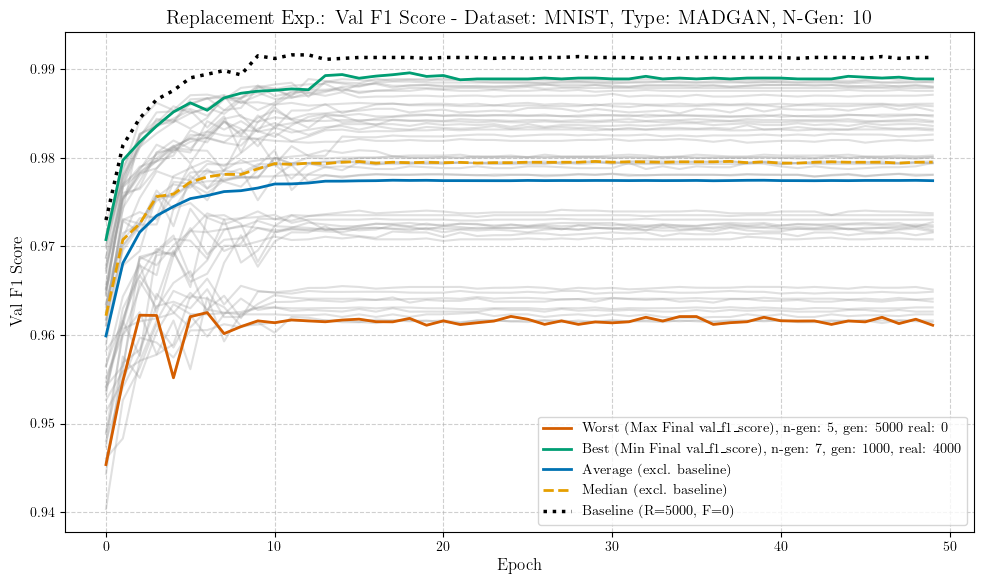
\includegraphics[width=\textwidth]{abb/strat_classifier_performance/MNIST_STRATIFIED_CLASSIFIERS_MADGAN_NEW/replacement_experiments/val_f1_score_MADGAN_MNIST_n_gen_10_all.png}
		\caption{F1 Score on MNIST over 50 epochs. Augmentation technique: MADGAN (K=10)}
        \label{fig:res_replacement_mnist_tda_vs_madgan__madgan}
	\end{subfigure}
	\begin{subfigure}{.85\textwidth}
		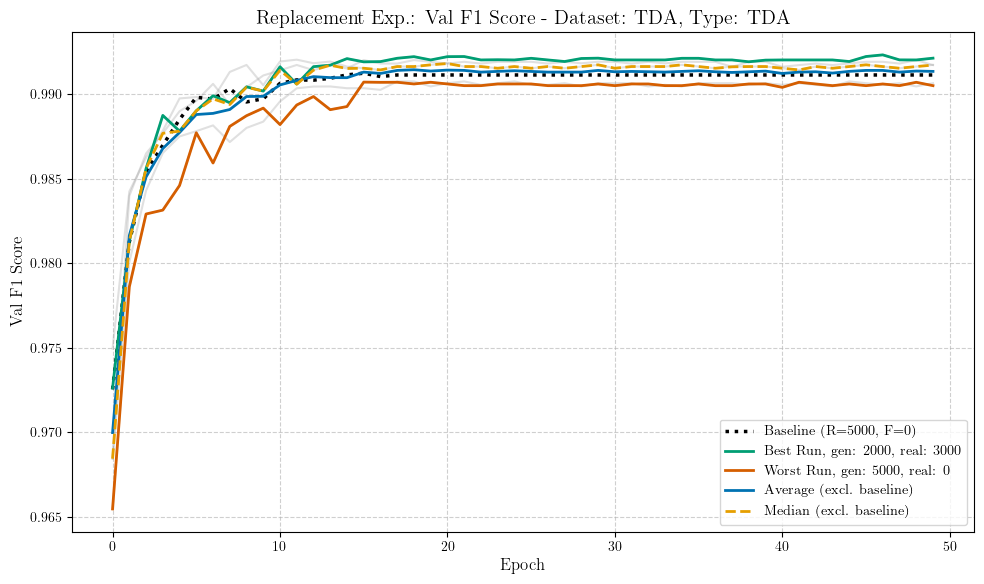
\includegraphics[width=\textwidth]{abb/strat_classifier_performance/tda_mnist/replacement_experiments/val_f1_score_tda_mnist_mnist_all.png}
		\caption{F1 Score on MNIST over 50 epochs. Augmentation Technique: TDA}
        \label{fig:res_replacement_mnist_tda_vs_madgan__tda}
	\end{subfigure}
%%%%%%%%%%%%%%
\end{figure}

\begin{table}[H]
	\vspace{-1.5em}
	\centering
	\begin{tabular}{|c|c|c|c|}
		\hline
		Run Type & Experiment & Val F1 \\ \hline
		best & \(G_{10, 7}\), R:4000, F:1000 & $0.9889$\\ \hline
		worst & \(G_{10, 5}\), R:0, F:5000 & $0.9611$\\ \hline
		median & G (K=10) & $0.9795$\\ \hline
		average & G (K=10) & $0.9774$
		\\ \hline
	\end{tabular}
    \caption{Final F1 Scores after 50 epochs. Augmentation technique: MADGAN}
        \label{tab:res_replacement_mnist_tda_vs_madgan__madgan}
\end{table}
\begin{table}[H]
	\centering
	\vspace{-1.5em}
	\begin{tabular}{|c|c|c|c|c|}
		\hline
		Run Type & Metric & Val F1 \\ \hline
		best & TDA, R:3000, F:2000 & $0.9922$\\ \hline
		worst & TDA, R:0, F:5000 & $0.9905$\\ \hline
		median & TDA & $0.9917$\\ \hline
		average & TDA & $0.9914$
		\\ \hline
	\end{tabular}
    \caption{Final F1 Scores after 50 epochs. Augmentation technique: TDA}
        \label{tab:res_replacement_mnist_tda_vs_madgan__tda}
\end{table}

All graphs in the corresponding figure show rapid convergence and stable training 15 epochs. After 20 epochs, only small fluctuations in the result can be seen for both TDA and MADGAN GDA. With a small spread of $0.0017$, all ratios for the TDA resulted in a F1 score, on the validation set of over $0.99$. This allows the conclusion that replacing training images for a classifier with modified images results in minimal negative impact on their performance, measured on the validation set using the F1 score. It is important to emphasize, that the best, median and average measured surpassed the baseline, leading to the fact that the augmentation improved the classifiers' performance on average.

The best performing setting on MNIST for MADGAN is with $K=10$. Showing a similar fast convergence compared to TDA, the MADGAN-augmented classifiers are mostly converged after the 15th epoch. In contrast to the TDA classifiers however, the performance using MADGAN images resulted in a significantly wider spread of classifier performances, of $0.0278$. It is critical to mention again, that Figure \ref{fig:res_replacement_mnist_tda_vs_madgan__madgan} shows performances across all ten generators, over all replacement ratios. This results in a total of $60$ classifiers trained. Generally, the graphs converge to lower F1 scores, compared to the classifiers utilizing TDA. Here, it can be concluded, that the average and median performance suffered from replacing the real images with generated images. The summary table quantifies this fact: the average final F1 score across ratios and generators is $0.9775$, which is significantly lower than the average of the traditional augmentation. While the best setup (\(G_{10,7}, R:4000, F:1000\)) reached a good score: $0.9889$; it is lower than the average performance across the different ratios in the TDA experiment. Even the worst performing classifier in the TDA experiment is better than the best score for GDA in this case.

In direct comparison, the TDA consistently outperforms GDA (with its best resulting setting, MADGAN (K=10)) in this replacement scenario. Replacing the real data with synthetic lead to a noticeable degradation of the classifiers' performance on the validation set. Taking the results from question 1 into account (\ref{exp_results_ans_q1}), even the MADGAN setup resulting in the best FID score are not as effective as traditional augmented real data, when substituting the real samples in the training set.

\newpage
\noindent\textbf{Expansion Experiment, Dataset: MNIST}
\begin{figure}[H]
	\centering
	\begin{subfigure}{.85\textwidth}
		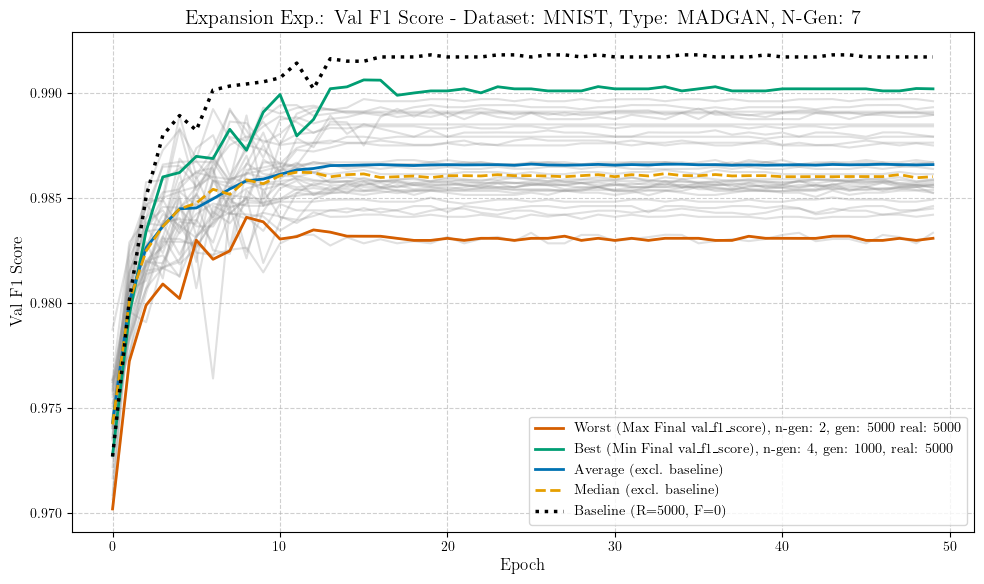
\includegraphics[width=\textwidth]{abb/strat_classifier_performance/MNIST_STRATIFIED_CLASSIFIERS_MADGAN_NEW/expansion_experiments/val_f1_score_MADGAN_MNIST_n_gen_7_all.png}
		\caption{F1 Score on MNIST over 50 epochs. Augmentation technique: MADGAN (K=7)}
        \label{fig:res_expansion_mnist_tda_vs_madgan__madgan}
	\end{subfigure}
	\begin{subfigure}{.85\textwidth}
		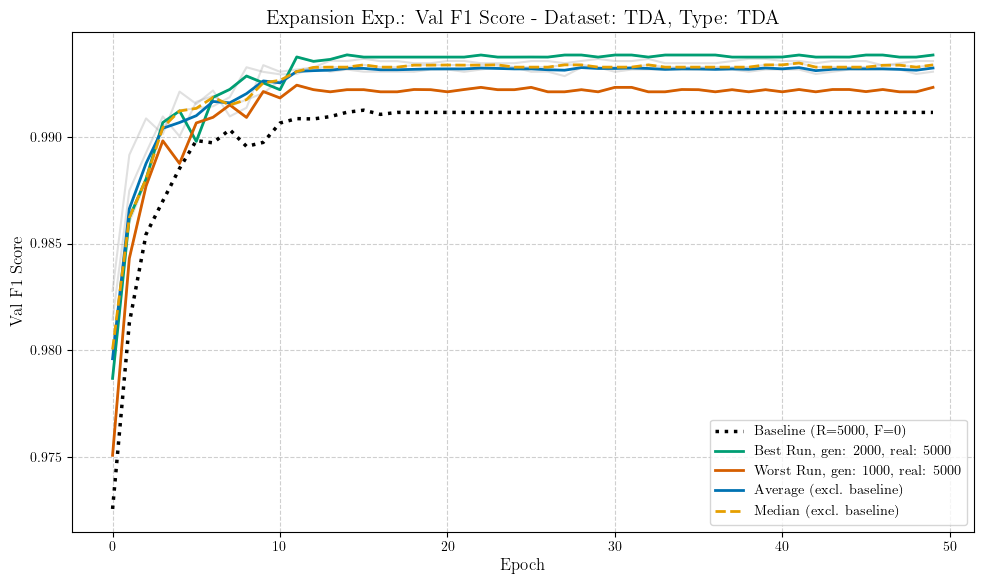
\includegraphics[width=\textwidth]{abb/strat_classifier_performance/tda_mnist/expansion_experiments/val_f1_score_tda_mnist_mnist_all.png}
		\caption{F1 Score on MNIST over 50 epochs. Augmentation Technique: TDA}
        \label{fig:res_expansion_mnist_tda_vs_madgan__tda}
	\end{subfigure}
%%%%%%%%%%%%%%
\end{figure}

\begin{table}[H]
	\vspace{-1.5em}
	\centering
	\begin{tabular}{|c|c|c|c|}
		\hline
		Run Type & Experiment & Val F1 \\ \hline
		best & \(G_{7, 4}\), R:5000, F:1000 & $0.9902$\\ \hline
		worst & \(G_{7, 2}\), R:5000, F:5000 & $0.9831$\\ \hline
		median & G (K=7) & $0.9860$\\ \hline
		average & G (K=7) & $0.9866$
		\\ \hline
	\end{tabular}
    \caption{Final F1 Scores after 50 epochs. Augmentation technique: MADGAN}
        \label{tab:res_expansion_mnist_tda_vs_madgan__madgan}
\end{table}
\begin{table}[H]
	\centering
	\vspace{-1.5em}
	\begin{tabular}{|c|c|c|c|c|}
		\hline
		Run Type & Experiment & Performance \\ \hline
		best & TDA, R:5000, F:2000 & $0.9938$\\ \hline
		worst & TDA, R:5000, F: 1000 & $0.9923$\\ \hline
		median & TDA & $0.9934$\\ \hline
		average & TDA & $0.9932$
		\\ \hline
	\end{tabular}
    \caption{Final F1 Scores after 50 epochs. Augmentation technique: TDA}
        \label{tab:res_expansion_mnist_tda_vs_madgan__tda}
\end{table}

The results using TDA (Table \ref{tab:res_expansion_mnist_tda_vs_madgan__tda}) show consistently high performance. The average final F1 score across all expansion levels (adding 0 to 5000 augmented samples per class) is $0.9932$, with minimal variation between the best ($0.9938$, achieved when adding 2000 augmented samples) and worst ($0.9923$) cases. This indicates that expanding the dataset with traditionally augmented samples maintains, and perhaps very slightly improves, the already high baseline performance on MNIST.

In contrast, using GDA with samples generated by the MADGAN (K=7) model did not yield performance improvements over the baseline trained only on real data. To be noted explicitly, none of the expansion experiments using MADGAN GDA surpassed the baseline performance level (see: \ref{app_strat_class_performance_madgan_mnist}). The summary statistics in Table \ref{tab:res_expansion_mnist_tda_vs_madgan__madgan}, which cover results across all 7 generators and all expansion ratios, confirm this. The average final F1 score is 0.9866, noticeably lower than the TDA results. The best-performing run across all generators and expansion levels only reached $0.9902$ (using generator \(G_{7,4}\) when adding 1000 synthetic samples), which is below even the worst TDA result. Performance tended to decrease as more synthetic data was added, with the lowest score ($0.9831$) occurring when the maximum of 5000 synthetic samples per class were added (using generator \(G_{7,2}\)).

Comparing the two augmentation strategies in the expansion scenario, TDA is clearly superior on MNIST in this setup. Expanding the dataset with traditionally augmented data maintains excellent performance, whereas expanding with MADGAN-generated synthetic data fails to improve over the real-data baseline and leads to lower overall performance. This suggests that the synthetic samples from MADGAN (K=7), despite the model potentially having good generative scores, dilute rather than enhance the training data quality when added to the real MNIST dataset for this downstream classification task.

\newpage
\noindent\textbf{Replacement Experiment, Dataset: Fashion-MNIST}
\begin{figure}[H]
	\centering
	\begin{subfigure}{.85\textwidth}
		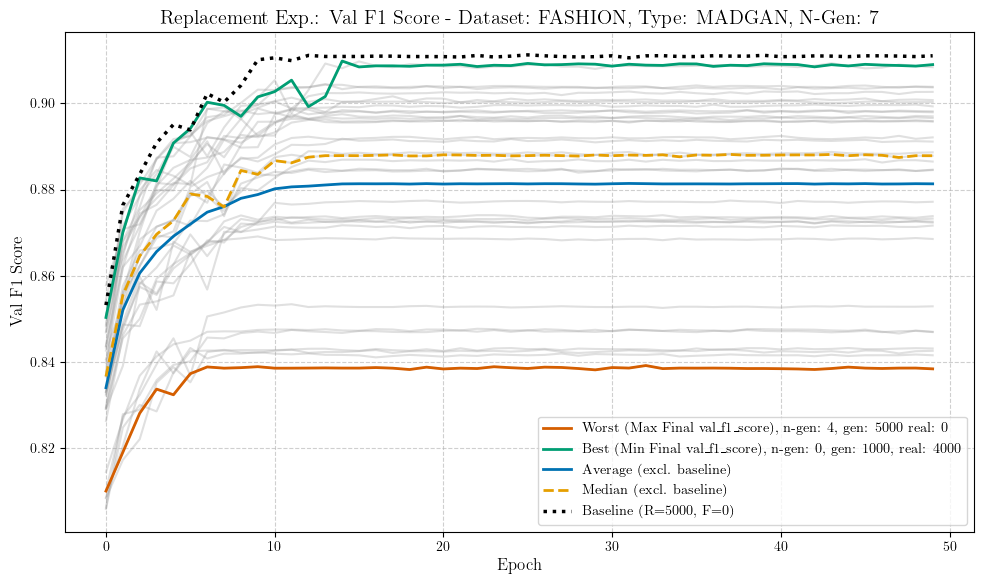
\includegraphics[width=\textwidth]{abb/strat_classifier_performance/FASHION_STRATIFIED_CLASSIFIERS_MADGAN_NEW/replacement_experiments/val_f1_score_MADGAN_FASHION_n_gen_7_all.png}
		\caption{F1 Score on FASHION over 50 epochs. Augmentation tech.: MADGAN (K=7)}
        \label{fig:res_replacement_fashion_tda_vs_madgan__madgan}
	\end{subfigure}
	\begin{subfigure}{.85\textwidth}
		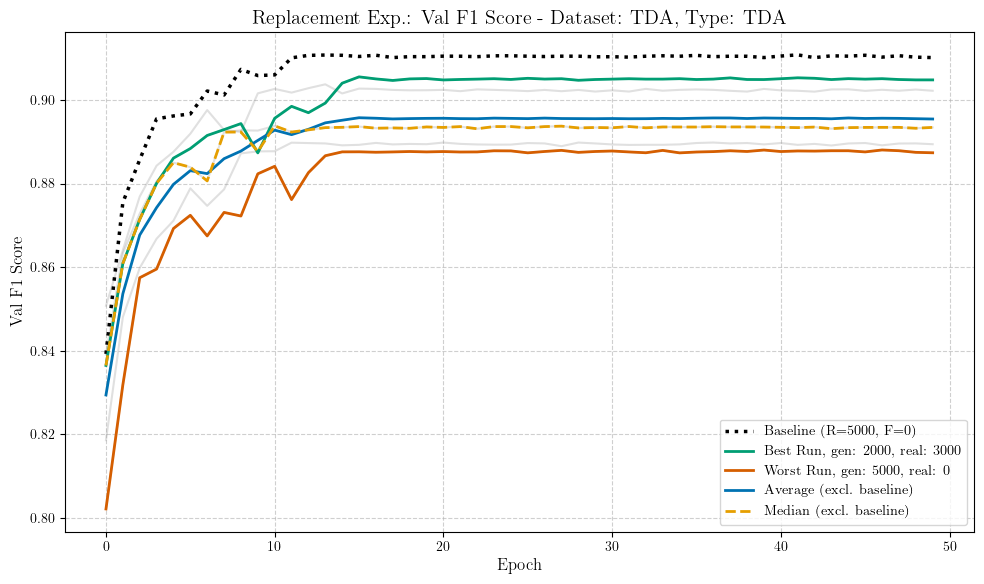
\includegraphics[width=\textwidth]{abb/strat_classifier_performance/tda_fashion_mnist/replacement_experiments/val_f1_score_tda_fashion_mnist_fashion_all.png}
		\caption{F1 Score on FASHION over 50 epochs. Augmentation Technique: TDA}
        \label{fig:res_replacement_fashion_tda_vs_madgan__tda}
	\end{subfigure}
%%%%%%%%%%%%%%
\end{figure}

\begin{table}[H]
	\vspace{-1.5em}
	\centering
	\begin{tabular}{|c|c|c|c|}
		\hline
		Run Type & Experiment & Val F1 \\ \hline
		best & \(G_{7, 0}\), R:4000, F:1000 & $0.9090$\\ \hline
		worst & \(G_{7, 4}\), R:0, F:5000 & $0.8384$\\ \hline
		median & G (K=7) & $0.8879$\\ \hline
		average & G (K=7) & $0.8813$
		\\ \hline
	\end{tabular}
    \caption{Final F1 Scores after 50 epochs. Augmentation tech.: MADGAN (K=7)}
        \label{tab:res_replacement_fashion_tda_vs_madgan__madgan}
\end{table}
\begin{table}[H]
	\centering
	\vspace{-1.5em}
	\begin{tabular}{|c|c|c|c|c|}
		\hline
		Run Type & Experiment & Val F1 \\ \hline
		best & TDA, R:3000, F:2000 & $0.9048$\\ \hline
		worst & TDA, R:0, F:5000 & $0.8874$\\ \hline
		median & TDA & $0.8934$\\ \hline
		average & TDA & $0.8955$
		\\ \hline
	\end{tabular}
    \caption{Final F1 Scores after 50 epochs. Augmentation technique: TDA}
        \label{tab:res_replacement_fashion_tda_vs_madgan__tda}
\end{table}

For Traditional Data Augmentation (TDA), as shown in Table \ref{tab:res_replacement_fashion_tda_vs_madgan__tda}, the classifier performance remains reasonably strong and relatively stable even as real data is substituted with traditionally augmented samples. Across all replacement ratios, the average final F1 score was $0.8955$. Performance experienced only a moderate decline with increasing replacement, peaking at $0.9048$ with a mix of 3000 real and 2000 augmented samples per class, and bottoming at $0.8874$ when relying solely on 5000 augmented samples. The narrow performance range underscores the consistency offered by TDA.

The MADGAN (K=7) GDA results, detailed in Table \ref{tab:res_replacement_fashion_tda_vs_madgan__madgan}, present a more varied picture. Notably, MADGAN GDA achieved a peak F1 score of $0.9090$ (from generator \(G_{7,0}\) with 4000 real and 1000 synthetic samples), which slightly surpasses the best performance seen with TDA. However, this potential for high performance is coupled with greater variability. The least favorable outcome for MADGAN GDA (generator \(G_{7,4}\) using only its 5000 generated samples) yielded an F1 score of \(0.8384\). While this represents a notable decrease in performance, it still constitutes a marked improvement over previously observed lower-bound scenarios. This brings the MADGAN’s average F1 score to \(0.8813\), which, while closer to the TDA average, remains slightly below it. The median F1 score for MADGAN GDA (\(0.8879\)) is also marginally lower than TDA’s median (\(0.8934\)).

Directly comparing the replacement scenario on Fashion-MNIST, TDA continues to offer a more consistently reliable performance. While MADGAN GDA, with its best generator and limited replacement, demonstrates the capacity to achieve a slightly higher peak F1 score than TDA. However, TDA maintains better average, median, and notably, a better F1 score under pessimistic condition. The synthetic data from some MADGAN generators, especially when used as a complete replacement for real data, leads to a more substantial performance degradation than observed with TDA, making TDA the more robust strategy overall for this replacement task, despite MADGAN's higher performance ceiling under optimal GDA conditions.

\newpage
\noindent\textbf{Expansion Experiment, Dataset: Fashion-MNIST}
\begin{figure}[H]
	\centering
	\begin{subfigure}{.85\textwidth}
		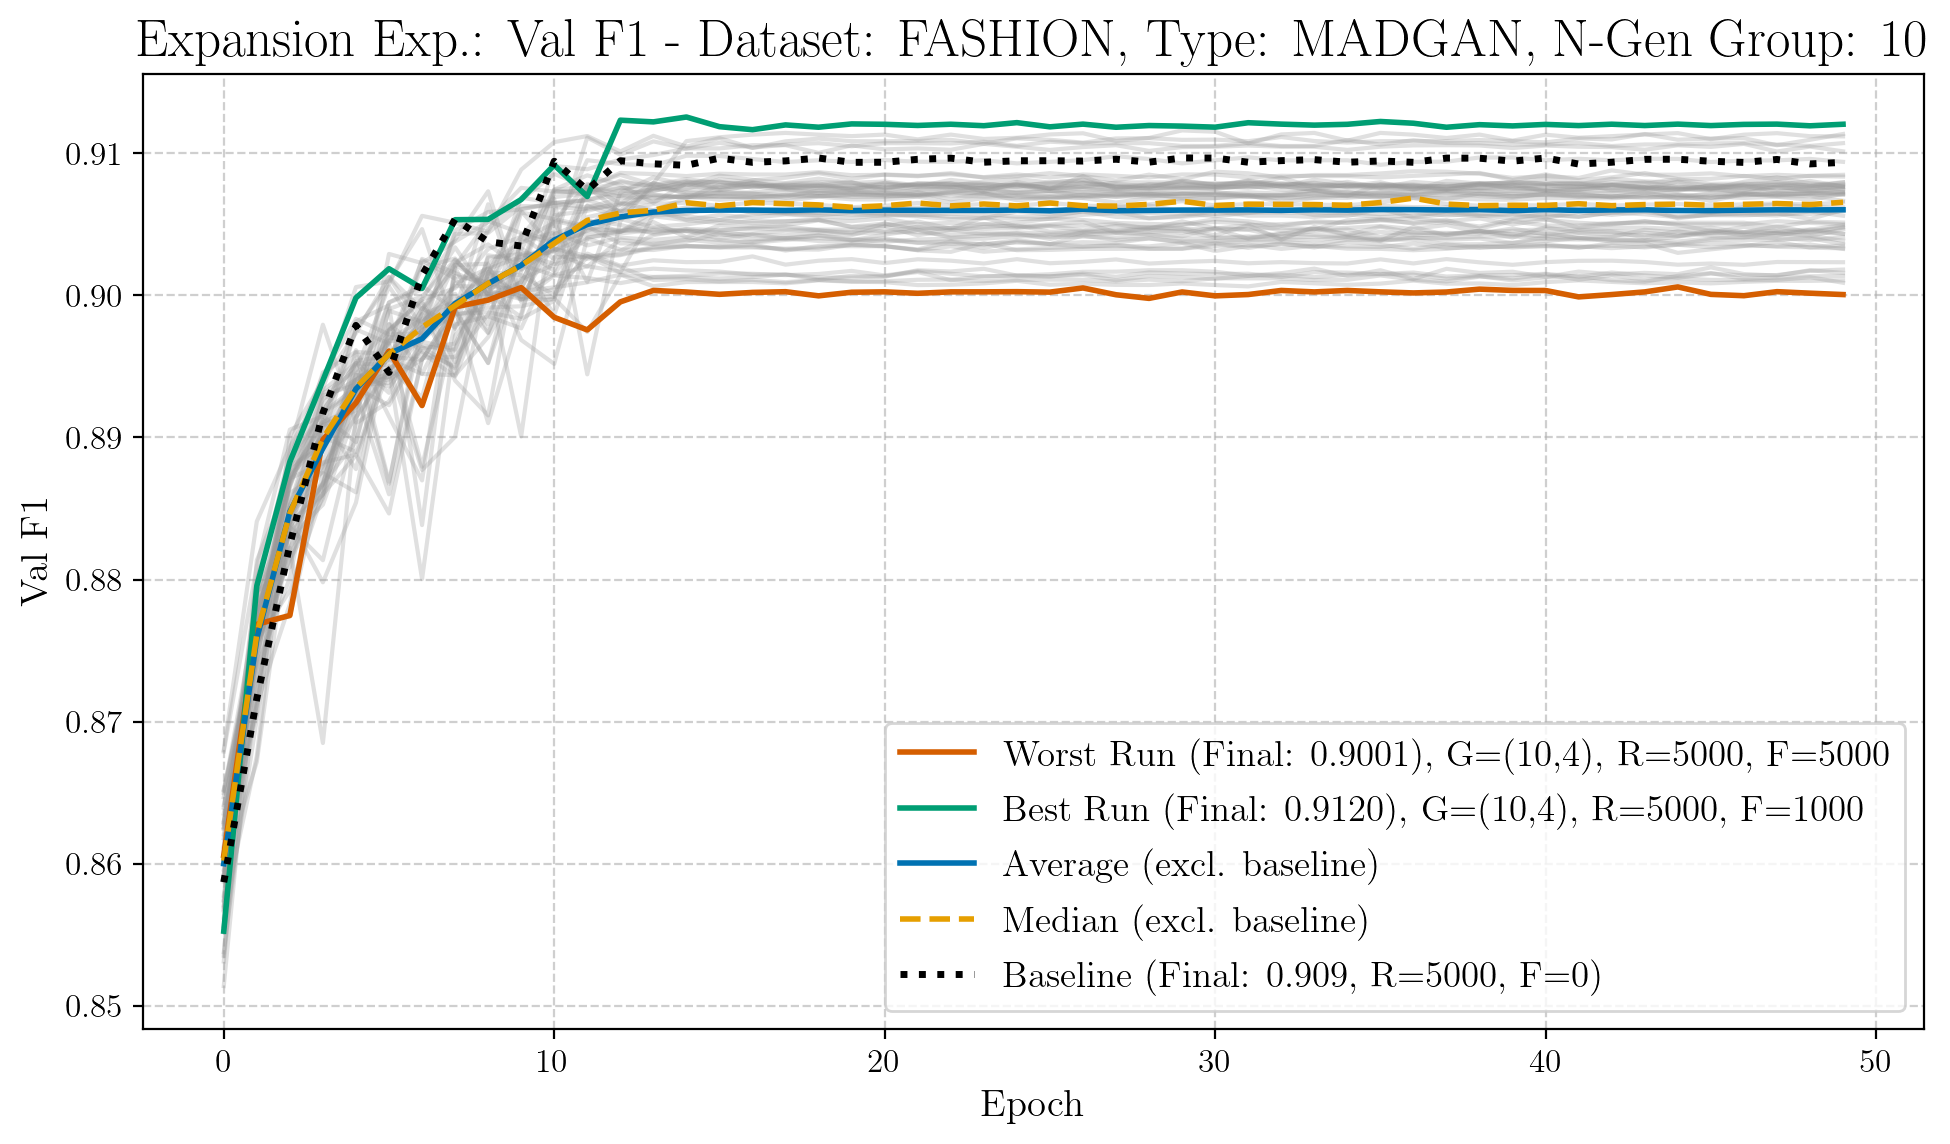
\includegraphics[width=\textwidth]{abb/strat_classifier_performance/FASHION_STRATIFIED_CLASSIFIERS_MADGAN_NEW/expansion_experiments/val_f1_score_MADGAN_FASHION_n_gen_10_all.png}
		\caption{F1 Score on FASHION over 50 epochs. Augmentation tech.: MADGAN (K=10)}
        \label{fig:res_expansion_fashion_tda_vs_madgan__madgan}
	\end{subfigure}
	\begin{subfigure}{.85\textwidth}
		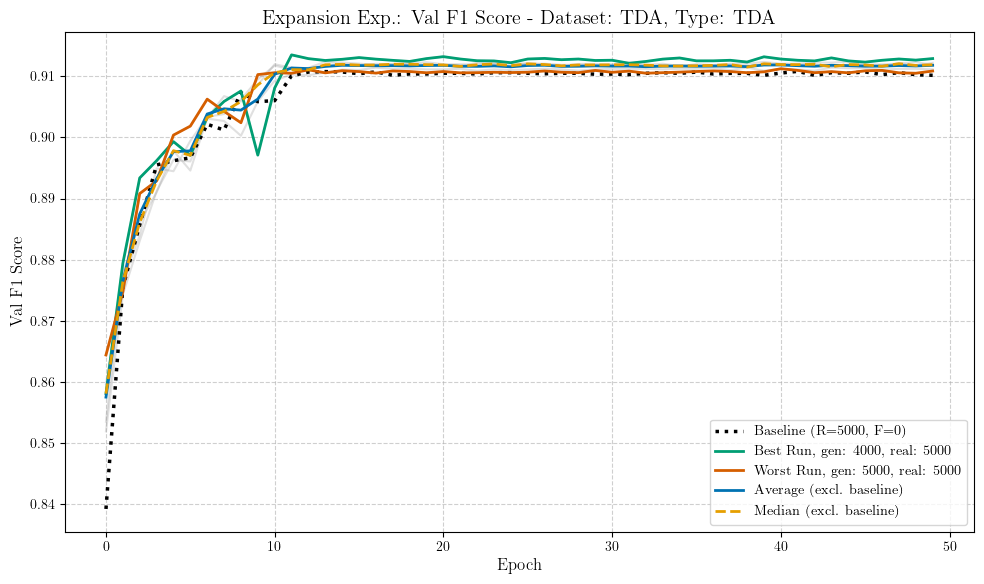
\includegraphics[width=\textwidth]{abb/strat_classifier_performance/tda_fashion_mnist/expansion_experiments/val_f1_score_tda_fashion_mnist_fashion_all.png}
		\caption{F1 Score on FASHION over 50 epochs. Augmentation Technique: TDA}
        \label{fig:res_expansion_fashion_tda_vs_madgan__tda}
	\end{subfigure}
%%%%%%%%%%%%%%
\end{figure}

\begin{table}[H]
	\vspace{-1.5em}
	\centering
	\begin{tabular}{|c|c|c|c|}
		\hline
		Run Type & Experiment & Val F1 \\ \hline
		best & \(G_{10, 4}\), R:5000, F:1000 & $0.9120$\\ \hline
		worst & \(G_{10, 4}\), R:5000, F:5000 & $0.9001$\\ \hline
		median & G (K=10) & $0.9066$\\ \hline
		average & (K=10) & $0.9060$
		\\ \hline
	\end{tabular}
    \caption{Final F1 Scores after 50 epochs. Augmentation tech.: MADGAN (K=10)}
        \label{tab:res_expansion_fashion_tda_vs_madgan__madgan}
\end{table}
\begin{table}[H]
	\centering
	\vspace{-1.5em}
	\begin{tabular}{|c|c|c|c|c|}
		\hline
		Run Type & Experiment & Val F1 \\ \hline
		best & TDA, R:5000, F:4000 & $0.9129$\\ \hline
		worst & TDA, R:5000, F:5000 & $0.9108$\\ \hline
		median & TDA & $0.9119$\\ \hline
		average & TDA & $0.9118$
		\\ \hline
	\end{tabular}
    \caption{Final F1 Scores after 50 epochs. Augmentation technique: TDA}
        \label{tab:res_expansion_fashion_tda_vs_madgan__tda}
\end{table}

Above results show, that data expansion on Fashion-MNIST is beneficial for both augmentation techniques. Unlike observations on MNIST, for which MADGAN GDA did not surpass the respective baseline. Utilizing TDA (Table \ref{tab:res_expansion_fashion_tda_vs_madgan__tda}) to add samples improves the classifiers performance over the baseline, achieving a peak F1 score of $0.9129$ when adding 4000 augmented samples to each class. The F1 performance remains high, despite varying ratios or real to fake images. The setting achieved an average F1 score of $0.9118$ and even the worst case (adding 5000 samples) scored $0.9108$.

On the Fashion-MNIST dataset, data expansion proved advantageous for both augmentation strategies, a notable contrast to earlier MNIST findings where MADGAN GDA struggled to exceed baseline performance. With Traditional Data Augmentation (TDA), as detailed in \ref{tab:res_expansion_fashion_tda_vs_madgan__tda}, incorporating additional augmented samples demonstrably boosted classifier F1 scores over the R:5000/F:0 baseline. This enhancement culminated in a peak F1 score of $0.9129$ with the addition of 4000 augmented samples per class. TDA maintained remarkably high and stable performance throughout the expansion, evidenced by an average F1 score of \(0.9118\) and a strong minimum observed score of \(0.9108\) even when 5000 augmented samples were added.


Generative Data Augmentation using MADGAN (K=10) also improved performance over the presumed baseline, as indicated by the summary statistics in \ref{tab:res_expansion_fashion_tda_vs_madgan__madgan}. Its best-case F1 score reached $0.9120$, achieved by generator \(G_{10,4}\) with an addition of 1000 synthetic samples per class, closely rivaling TDA's peak and underscoring GDA's effectiveness in this scenario. While this peak is promising, MADGAN GDA exhibited slightly less consistency than TDA. Its average F1 score ($0.9060$) and median ($0.9066$) were marginally lower than TDA's equivalents. Furthermore, performance showed a more pronounced decline when maximally expanded with 5000 synthetic samples, dropping to $0.9001$ in the worst run—a score notably below TDA's worst case. Nevertheless, the variability across MADGAN's generators and expansion ratios was considerably less extreme than what was observed in the Fashion-MNIST replacement experiments.

Ultimately, for data expansion on Fashion-MNIST, both TDA and MADGAN GDA (K=10) offered tangible benefits over relying solely on the original real data. TDA, however, maintained a slight overall advantage, delivering marginally higher peak performance ($0.9129$ for TDA vs. $0.9120$ for MADGAN GDA) and superior stability, particularly evident when large volumes of augmented data were incorporated. While MADGAN GDA proved highly competitive by nearly matching TDA's peak, its slightly lower average scores and more significant performance drop under maximum expansion conditions indicate that TDA remains the more robust expansion technique in this specific setup, though MADGAN GDA is clearly a viable alternative.


\newpage
\subsubsection[Question 3]{MADGAN GDA vs. Deep Convolutional/Conditional GAN GDA} \label{exp_results_ans_q3}
In the foregoing chapter (\ref{exp_results_ans_q2}), the most successful setting for the MADGAN architecture has been set. MADGAN with K=10 for Replacement-, with K=7 for the Expansion scenario on MNIST and for Fashion-MNIST K=7 for Replacement- and K=10 for Expansion proved to perform best under given circumstances. Following, the same settings for the respective dataset and the corresponding experimental setup (replacement, expansion) will be used to compare against the best performing architecture of deep convolutional and conditional GANs. For both, the Replacement and Expansion scenario, the cGAN surpassed the performance of the DCGAN. Thus, the cGAN is selected for direct comparison. The DCGAN will only be described and linked were fit.

% TODO: preamble the results of the following experiments
\newpage

\noindent\textbf{Replacement Experiment, Dataset: MNIST}
\begin{figure}[H]
	\centering
	\begin{subfigure}{.85\textwidth}
		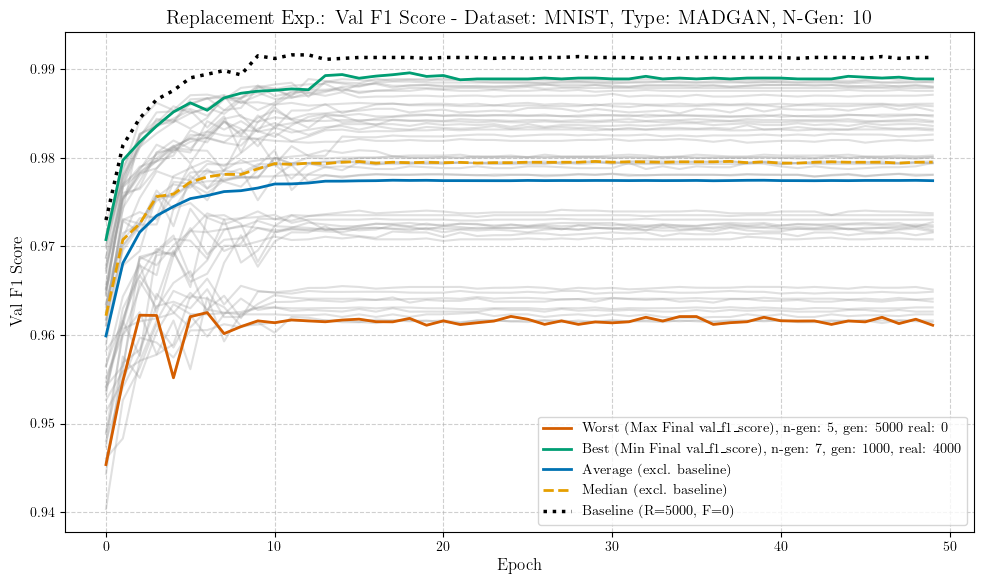
\includegraphics[width=\textwidth]{abb/strat_classifier_performance/MNIST_STRATIFIED_CLASSIFIERS_MADGAN_NEW/replacement_experiments/val_f1_score_MADGAN_MNIST_n_gen_10_all.png}
		\caption{F1 Score on MNIST over 50 epochs. Augmentation technique: MADGAN (K=10)}
        \label{fig:res_replacement_mnist_ccgan_vs_madgan__madgan}
	\end{subfigure}
	\begin{subfigure}{.85\textwidth}
		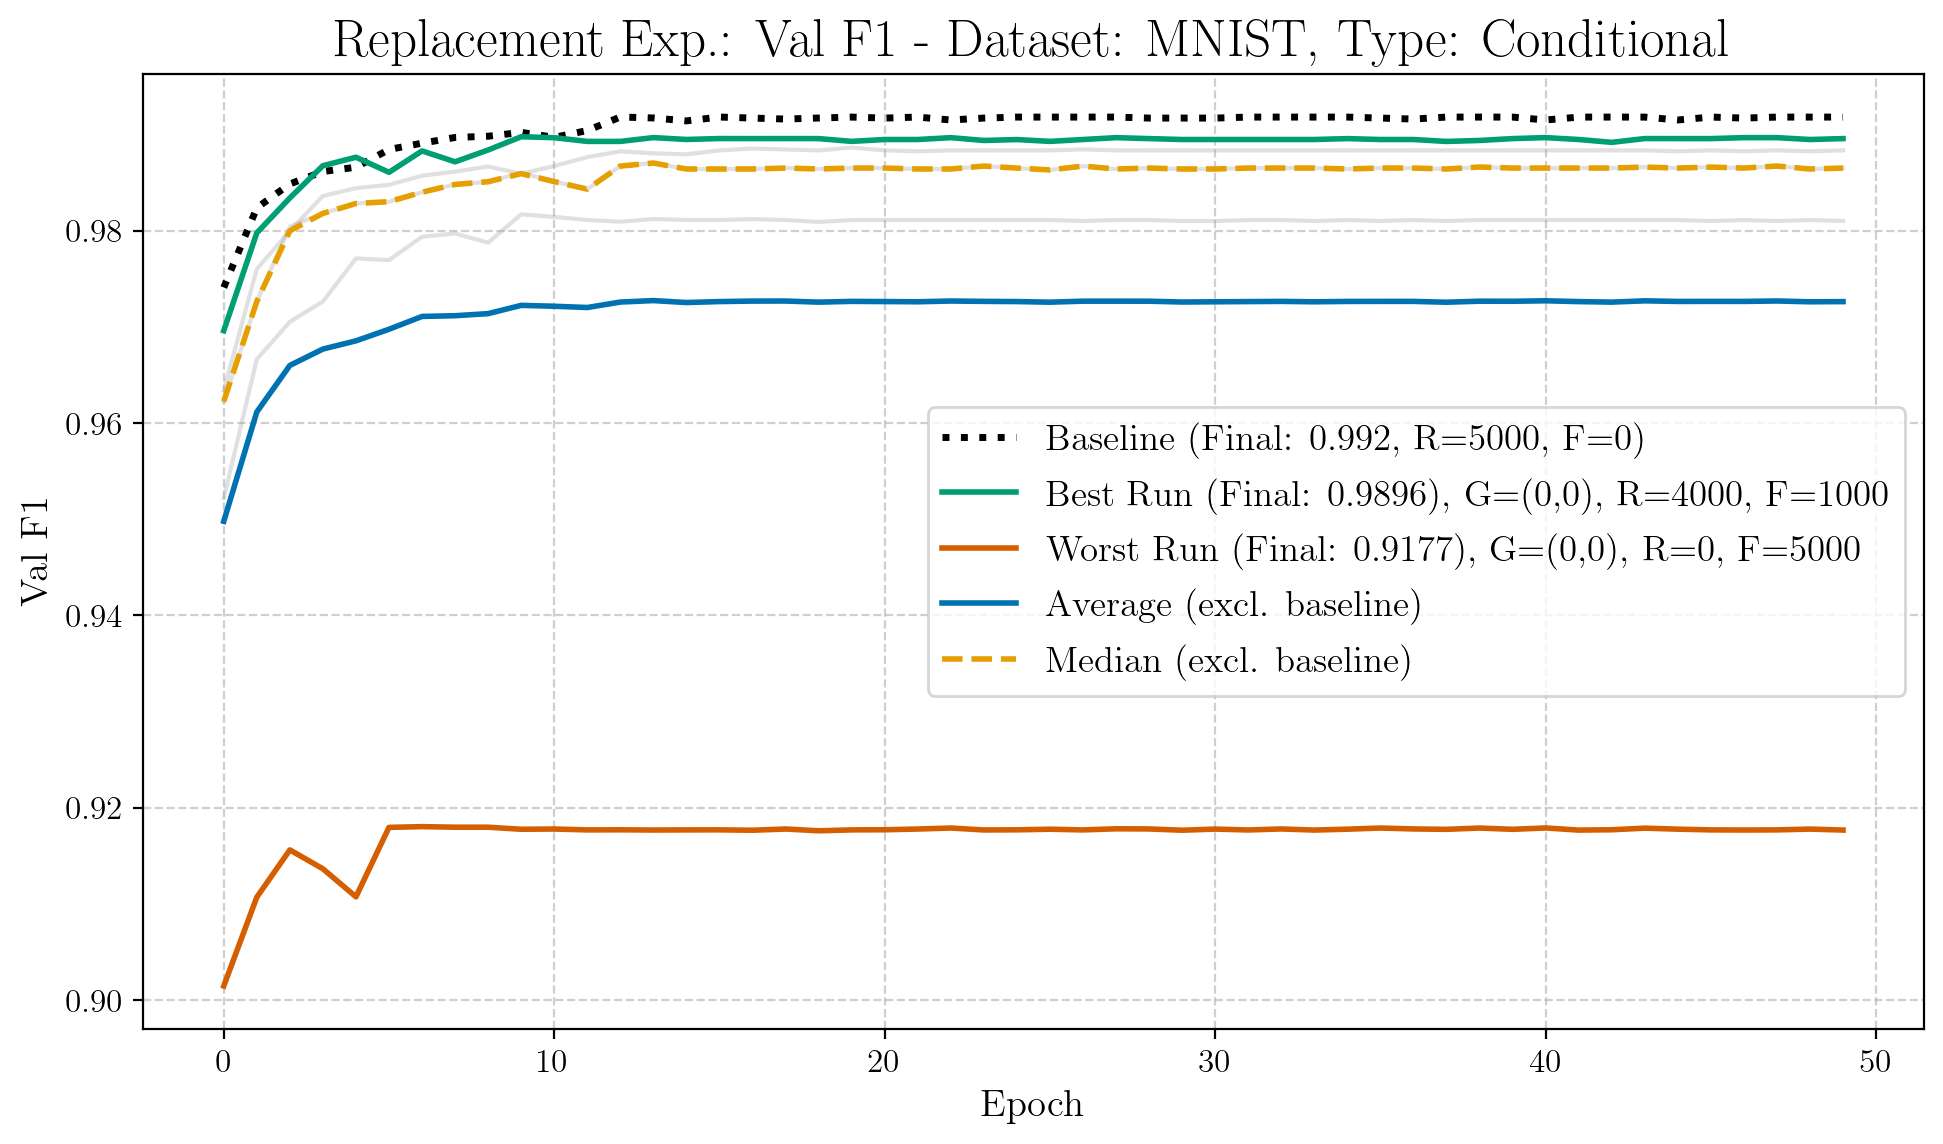
\includegraphics[width=\textwidth]{abb/strat_classifier_performance/MNIST_STRATIFIED_CLASSIFIERS_COND_GAN/replacement_experiments/val_f1_score_['COND']_MNIST_all.png}
		\caption{F1 Score on MNIST over 50 epochs. Augmentation Technique: cGAN}
        \label{fig:res_replacement_mnist_ccgan_vs_madgan__cgan}
	\end{subfigure}
%%%%%%%%%%%%%%
\end{figure}

\begin{table}[H]
	\vspace{-1.5em}
	\centering
	\begin{tabular}{|c|c|c|c|}
		\hline
		Run Type & Experiment & Val F1 \\ \hline
		best & \(G_{10, 7}\), R:4000, F:1000 & $0.9889$\\ \hline
		worst & \(G_{10, 5}\), R:0, F:5000 & $0.9611$\\ \hline
		median & G (K=10) & $0.9795$\\ \hline
		average & G (K=10) & $0.9774$
		\\ \hline
	\end{tabular}
    \caption{Final F1 Scores after 50 epochs. Augmentation technique: MADGAN (K=10)}
        \label{tab:res_replacement_mnist_ccgan_vs_madgan__madgan}
\end{table}
\begin{table}[H]
	\centering
	\vspace{-1.5em}
	\begin{tabular}{|c|c|c|c|c|}
		\hline
		Run Type & Experiment & Val F1 \\ \hline
		best & Conditional, R:4000, F:1000 & $0.9896$\\ \hline
		worst & Conditional, R:0, F:5000 & $0.9177$\\ \hline
		median & Conditional & $0.9865$\\ \hline
		average & Conditional & $0.9726$
		\\ \hline
	\end{tabular}
    \caption{Final F1 Scores after 50 epochs. Augmentation technique: cGAN}
        \label{tab:res_replacement_mnist_ccgan_vs_madgan__cgan}
\end{table}
Both MADGAN (K=10) and cGAN demonstrate strong peak performance when replacing only a small amount of real data. As shown in Tables \ref{tab:res_replacement_mnist_ccgan_vs_madgan__madgan} and \ref{tab:res_replacement_mnist_ccgan_vs_madgan__cgan}, the best F1 scores achieved are very similar, with cGAN reaching $0.9896$ and MADGAN K=10 reaching $0.9889$, both occurring when 1000 real samples per class were replaced with synthetic ones (R:4000, F:1000).

However, the two methods exhibit different robustness levels as more real data is replaced. The cGAN performance degrades significantly when relying entirely on synthetic data (R:0, F:5000), with the F1 score dropping to $0.9177$. In contrast, the MADGAN (K=10) framework shows greater resilience in the purely synthetic scenario; even the worst-performing generator (\(G_{10,5}\)) at full replacement achieved an F1 score of $0.9611$, considerably higher than cGAN's worst score.

This difference in the weakest performance impacts the overall statistics. While cGAN achieves a higher median F1 score ($0.9865$) compared to MADGAN K=10 ($0.9795$), suggesting better typical performance across intermediate replacement ratios, MADGAN K=10 achieves a slightly higher average F1 score ($0.9774$ vs. $0.9726$ for cGAN). This is because MADGAN's performance does not drop as drastically as cGAN's in the full replacement scenario. Consequently, cGAN exhibits a larger overall performance range (spread of ~$0.072$) compared to MADGAN K=10 (spread of ~$0.028$) in this replacement experiment.

In conclusion, when replacing real MNIST data, both cGAN and MADGAN (K=10) GDA achieve similar high peak performance with limited replacement. However, MADGAN (K=10) demonstrates superior robustness when large amounts of real data are substituted, particularly in the scenario using only synthetic data. While cGAN performs slightly better across median replacement ratios, its sharp decline in the full synthetic setting makes MADGAN (K=10) appear more consistent overall in this specific replacement task, yielding a slightly better average F1 score.
\newpage
\noindent\textbf{Expansion Experiment, Dataset: MNIST}
\begin{figure}[H]
	\centering
	\begin{subfigure}{.85\textwidth}
		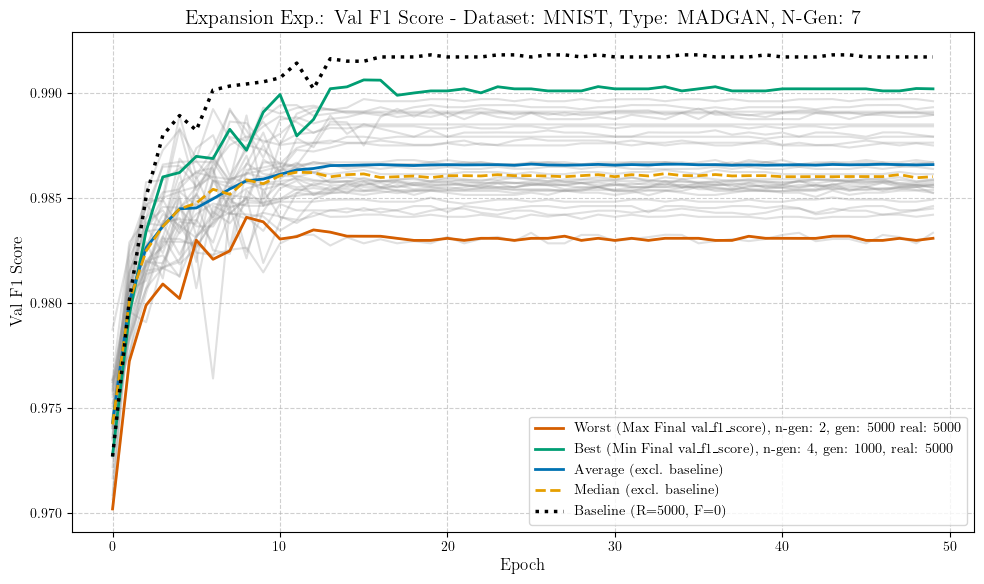
\includegraphics[width=\textwidth]{abb/strat_classifier_performance/MNIST_STRATIFIED_CLASSIFIERS_MADGAN_NEW/expansion_experiments/val_f1_score_MADGAN_MNIST_n_gen_7_all.png}
		\caption{F1 Score on MNIST over 50 epochs. Augmentation technique: MADGAN (K=7)}
        \label{fig:res_expansion_mnist_ccgan_vs_madgan__madgan}
	\end{subfigure}
	\begin{subfigure}{.85\textwidth}
		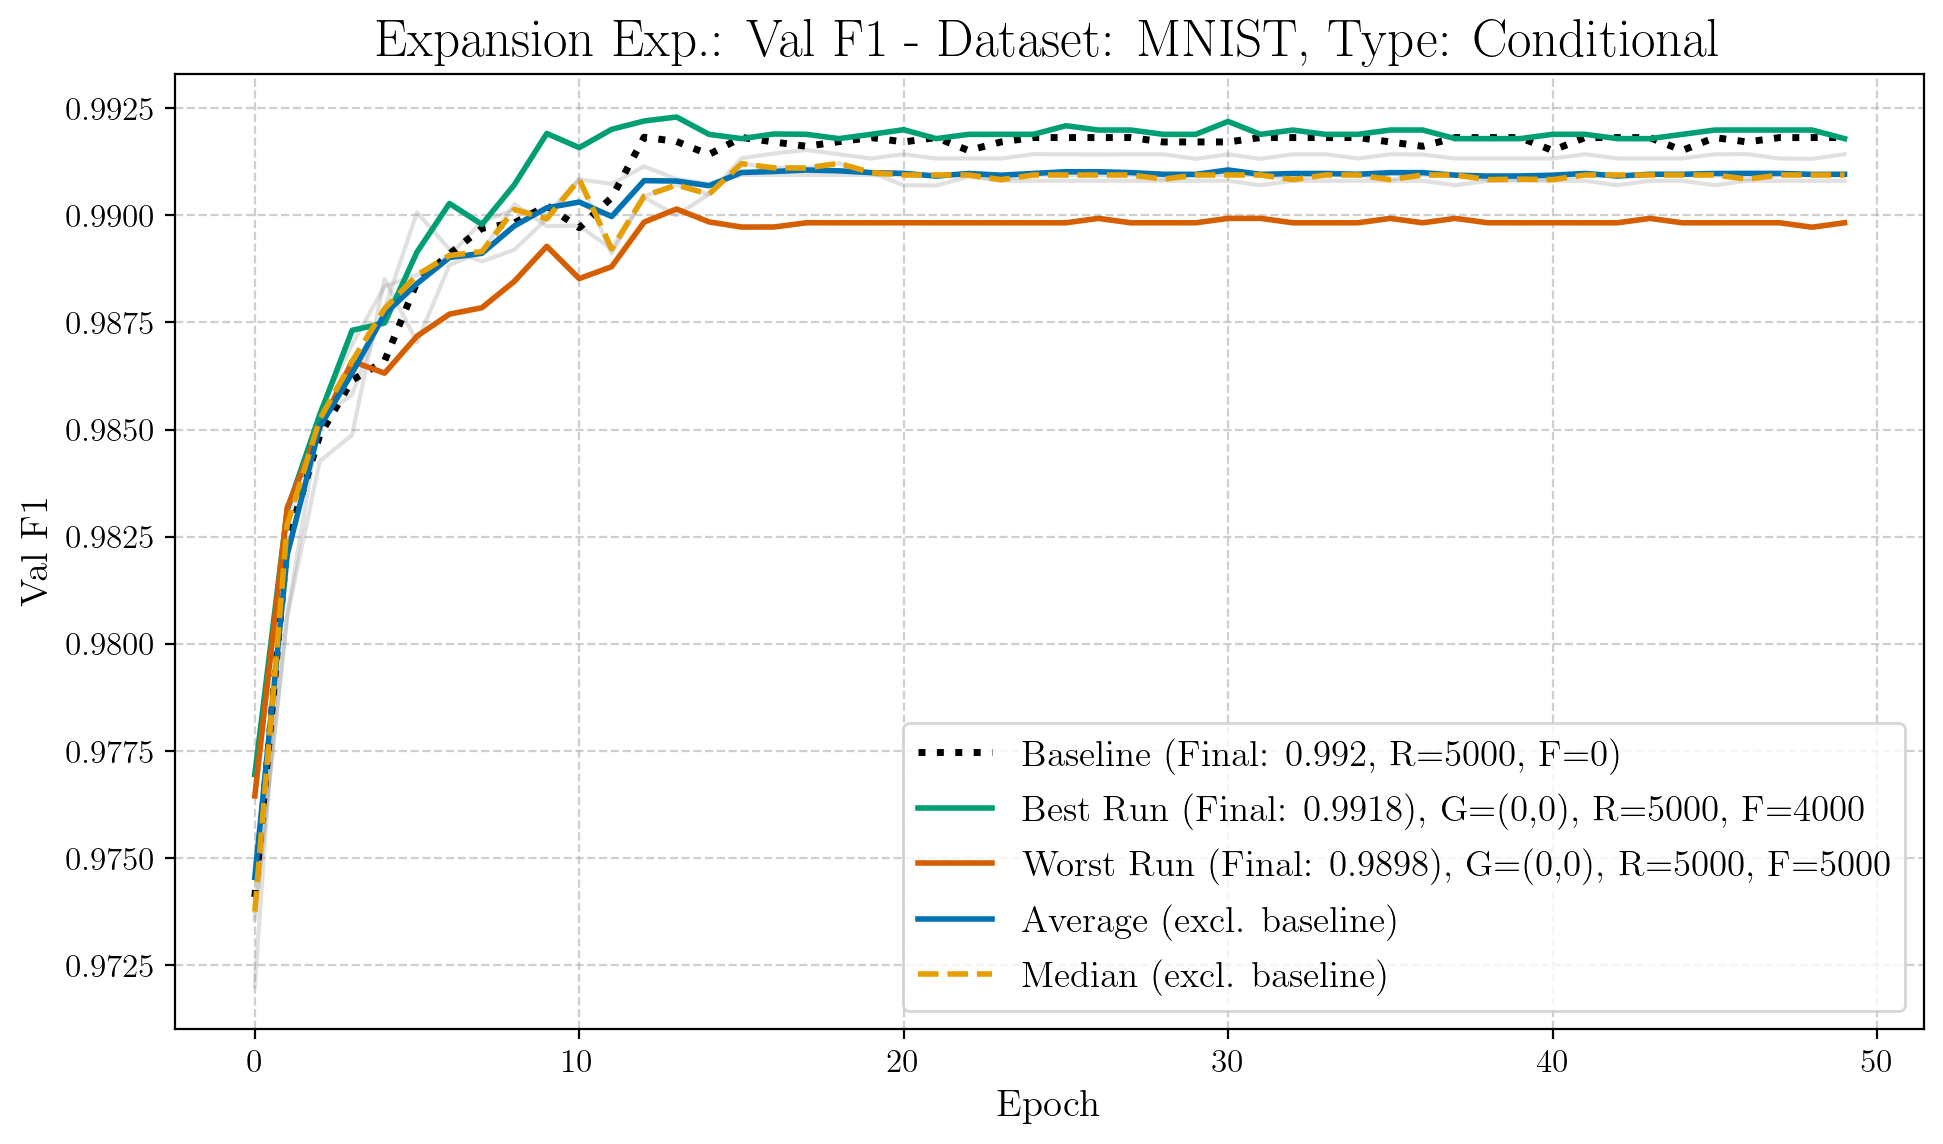
\includegraphics[width=\textwidth]{abb/strat_classifier_performance/MNIST_STRATIFIED_CLASSIFIERS_COND_GAN/expansion_experiments/val_f1_score_['COND']_MNIST_all.png}
		\caption{F1 Score on MNIST over 50 epochs. Augmentation Technique: cGAN}
        \label{fig:res_expansion_mnist_ccgan_vs_madgan__cgan}
	\end{subfigure}
%%%%%%%%%%%%%%
\end{figure}

\begin{table}[H]
	\vspace{-1.5em}
	\centering
	\begin{tabular}{|c|c|c|c|}
		\hline
		Run Type & Experiment & Val F1 \\ \hline
		best & \(G_{7, 4}\), R:5000, F:1000 & $0.9902$\\ \hline
		worst & \(G_{7, 2}\), R:5000, F:5000 & $0.9831$\\ \hline
		median & G (K=7) & $0.9860$\\ \hline
		average & G (K=7) & $0.9866$
		\\ \hline
	\end{tabular}
    \caption{Final F1 Scores after 50 epochs. Augmentation technique: MADGAN (K=10)}
        \label{tab:res_expansion_mnist_ccgan_vs_madgan__madgan}
\end{table}
\begin{table}[H]
	\centering
	\vspace{-1.5em}
	\begin{tabular}{|c|c|c|c|c|}
		\hline
		Run Type & Experiment & Val F1 \\ \hline
		best & Conditional, R:5000, F:4000 & $0.9918$\\ \hline
		worst & Conditional, R:5000, F:5000 & $0.9898$\\ \hline
		median & Conditional & $0.9909$\\ \hline
		average & Conditional & $0.9910$
		\\ \hline
	\end{tabular}
    \caption{Final F1 Scores after 50 epochs. Augmentation technique: cGAN}
        \label{tab:res_expansion_mnist_ccgan_vs_madgan__cgan}
\end{table}

The results clearly indicate that cGAN provides superior GDA performance compared to MADGAN (K=7) in this expansion scenario on MNIST. Examining the summary statistics, cGAN outperforms MADGAN K=7 across all metrics. The best F1 score achieved with cGAN ($0.9918$) is higher than MADGAN's best ($0.9902$). More significantly, cGAN maintains high performance even when the maximum number of synthetic samples are added (worst case F1 $0.9898$), whereas MADGAN's lower-bound performance drops considerably lower ($0.9831$).

This difference in robustness is reflected in the average and median scores. cGAN achieves an average F1 of $0.9910$ and a median of $0.9909$, both higher than MADGAN's average (0.9866) and median ($0.9860$). Furthermore, cGAN exhibits much lower variability across the different expansion ratios compared to the variability observed across MADGAN's generators and expansion ratios (cGAN range ~$0.002$ vs. MADGAN range ~$0.007$).

Consistent with the earlier comparison against TDA, neither GDA method appears to significantly surpass their respective baseline performance achieved with 5000 real images per class alone. However, cGAN maintains performance very close to this baseline level, while adding MADGAN (K=7) samples tends to result in slightly lower F1 scores.

Interestingly, taking the performance of the DCGAN into account (\ref{app_STRAT_CLASS_PERF_mnist_DCGAN}), it is clear, that its peak performance is in line with the highest score of the best MADGAN setup (K=7). The difference in peak F1 score is only $0.0005$ ($0.9889 - 0.9884$). Furthermore, the spread of performance is significantly smaller for the DCGAN.

In conclusion, for the task of expanding the MNIST training set, cGAN GDA is demonstrably more effective and stable than MADGAN (K=7) GDA. It achieves higher peak performance, maintains significantly better performance when large amounts of synthetic data are added, and exhibits less variability compared to the multi-generator approach in this configuration.

\newpage
\noindent\textbf{Replacement Experiment, Dataset: Fashion-MNIST}
\begin{figure}[H]
	\centering
	\begin{subfigure}{.85\textwidth}
		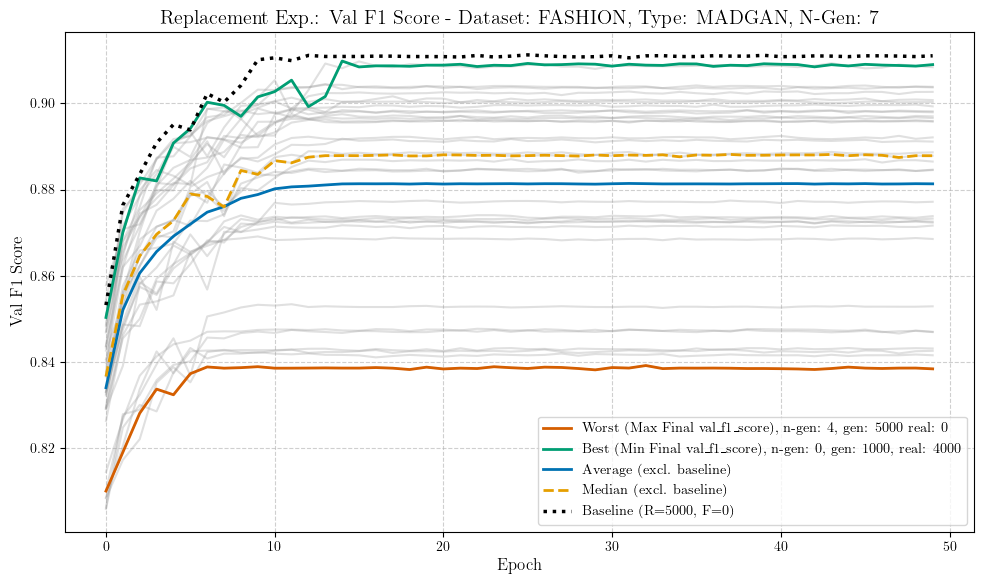
\includegraphics[width=\textwidth]{abb/strat_classifier_performance/FASHION_STRATIFIED_CLASSIFIERS_MADGAN_NEW/replacement_experiments/val_f1_score_MADGAN_FASHION_n_gen_7_all.png}
		\caption{F1 Score on FASHION over 50 epochs. Augmentation tech.: MADGAN (K=7)}
        \label{fig:res_replacement_fashion_cgan_vs_madgan__madgan}
	\end{subfigure}
	\begin{subfigure}{.85\textwidth}
		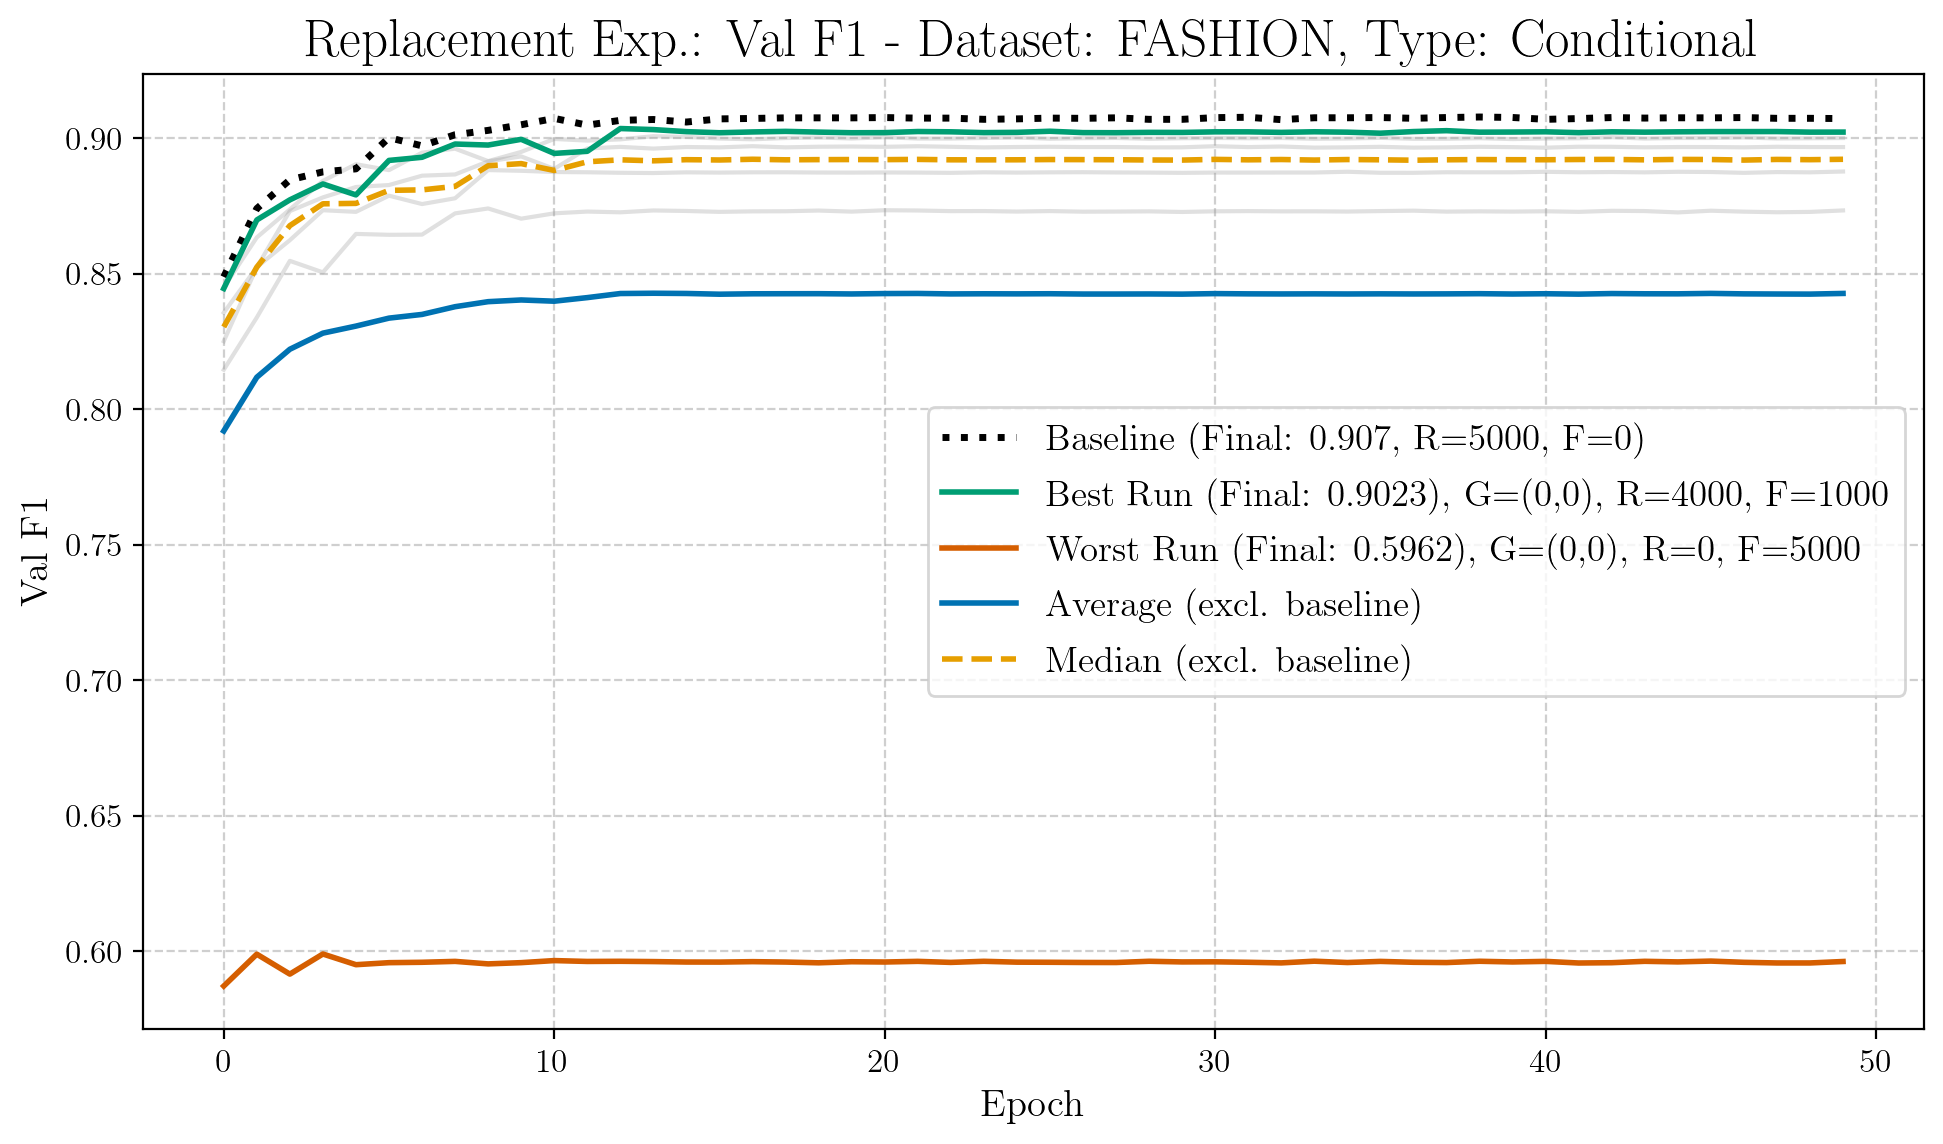
\includegraphics[width=\textwidth]{abb/strat_classifier_performance/FASHION_STRATIFIED_CLASSIFIERS_COND_GAN/replacement_experiments/val_f1_score_['COND']_FASHION_all.png}
		\caption{F1 Score on FASHION over 50 epochs. Augmentation Technique: cGAN}
        \label{fig:res_replacement_fashion_cgan_vs_madgan__cgan}
	\end{subfigure}
%%%%%%%%%%%%%%
\end{figure}

\begin{table}[H]
	\vspace{-1.5em}
	\centering
	\begin{tabular}{|c|c|c|c|}
		\hline
		Run Type & Experiment & Val F1 \\ \hline
		best & \(G_{7, 2}\), R:4000, F:1000 & $0.9079$\\ \hline
		worst & \(G_{7, 0}\), R:0, F:5000 & $0.3419$\\ \hline
		median & G = (K=7) & $0.8927$\\ \hline
		average & G = (K=7) & $0.7993$
		\\ \hline
	\end{tabular}
    \caption{Final F1 Scores after 50 epochs. Augmentation tech.: MADGAN (K=7)}
        \label{tab:res_replacement_fashion_cgan_vs_madgan__madgan}
\end{table}
\begin{table}[H]
	\centering
	\vspace{-1.5em}
	\begin{tabular}{|c|c|c|c|c|}
		\hline
		Run Type & Experiment & Val F1 \\ \hline
		best & Conditional R:4000, F:1000 & $0.9023$\\ \hline
		worst & Conditional R:0, F:5000 & $0.5962$\\ \hline
		median & Conditional & $0.8923$\\ \hline
		average & Conditional & $0.8427$
		\\ \hline
	\end{tabular}
    \caption{Final F1 Scores after 50 epochs. Augmentation technique: cGAN}
        \label{tab:res_replacement_fashion_cgan_vs_madgan__cgan}
\end{table}
Examining the peak performances, MADGAN (K=7) achieved a slightly higher best F1 score ($0.9079$ with generator \(G_{7,2}\) at R:4000, F:1000) compared to cGAN's best ($0.9023$ at the same replacement ratio). This suggests that, under optimal conditions (specific generator and limited replacement), MADGAN GDA can potentially offer a marginal advantage.

However, the performance when relying more heavily on synthetic data reveals significant differences in robustness. When all real data is replaced (R:0, F:5000), cGAN's F1 score drops to $0.5962$. While this is a substantial decrease, it is considerably better than the lowest result for MADGAN (K=7), where using only synthetic data from its poorest performing generator (\(G_{7,0}\)) resulted in an F1 score of just $0.3419$.

This disparity in pessimistic performance heavily influences the average scores. The cGAN achieves an average F1 score of $0.8427$ across all replacement ratios, which is notably higher than MADGAN K=7's average of $0.7993$. Interestingly, the median F1 scores are very similar ($0.8923$ for cGAN and 0.8927 for MADGAN K=7), indicating that the typical performance of both methods (excluding extreme outliers) is quite comparable. Nevertheless, MADGAN (K=7) exhibits a much larger overall spread in performance (range ~$0.566$) compared to cGAN (range $~0.306$), primarily due to its extremely low minimum scores.

In conclusion, for the replacement experiment on Fashion-MNIST, MADGAN (K=7) GDA can achieve a marginally higher peak F1 score than cGAN GDA with limited data replacement. That said, cGAN demonstrates greater robustness on average and provides a significantly better lower-bound performance when real data is fully substituted. The similar median scores suggest comparable typical performance, but MADGAN K=7 is less reliable overall due to the high variability among its individual generators, with some performing very poorly when used as the sole source of training data.

\newpage
\noindent\textbf{Expansion Experiment, Dataset: Fashion-MNIST}
\begin{figure}[H]
	\centering
	\begin{subfigure}{.85\textwidth}
		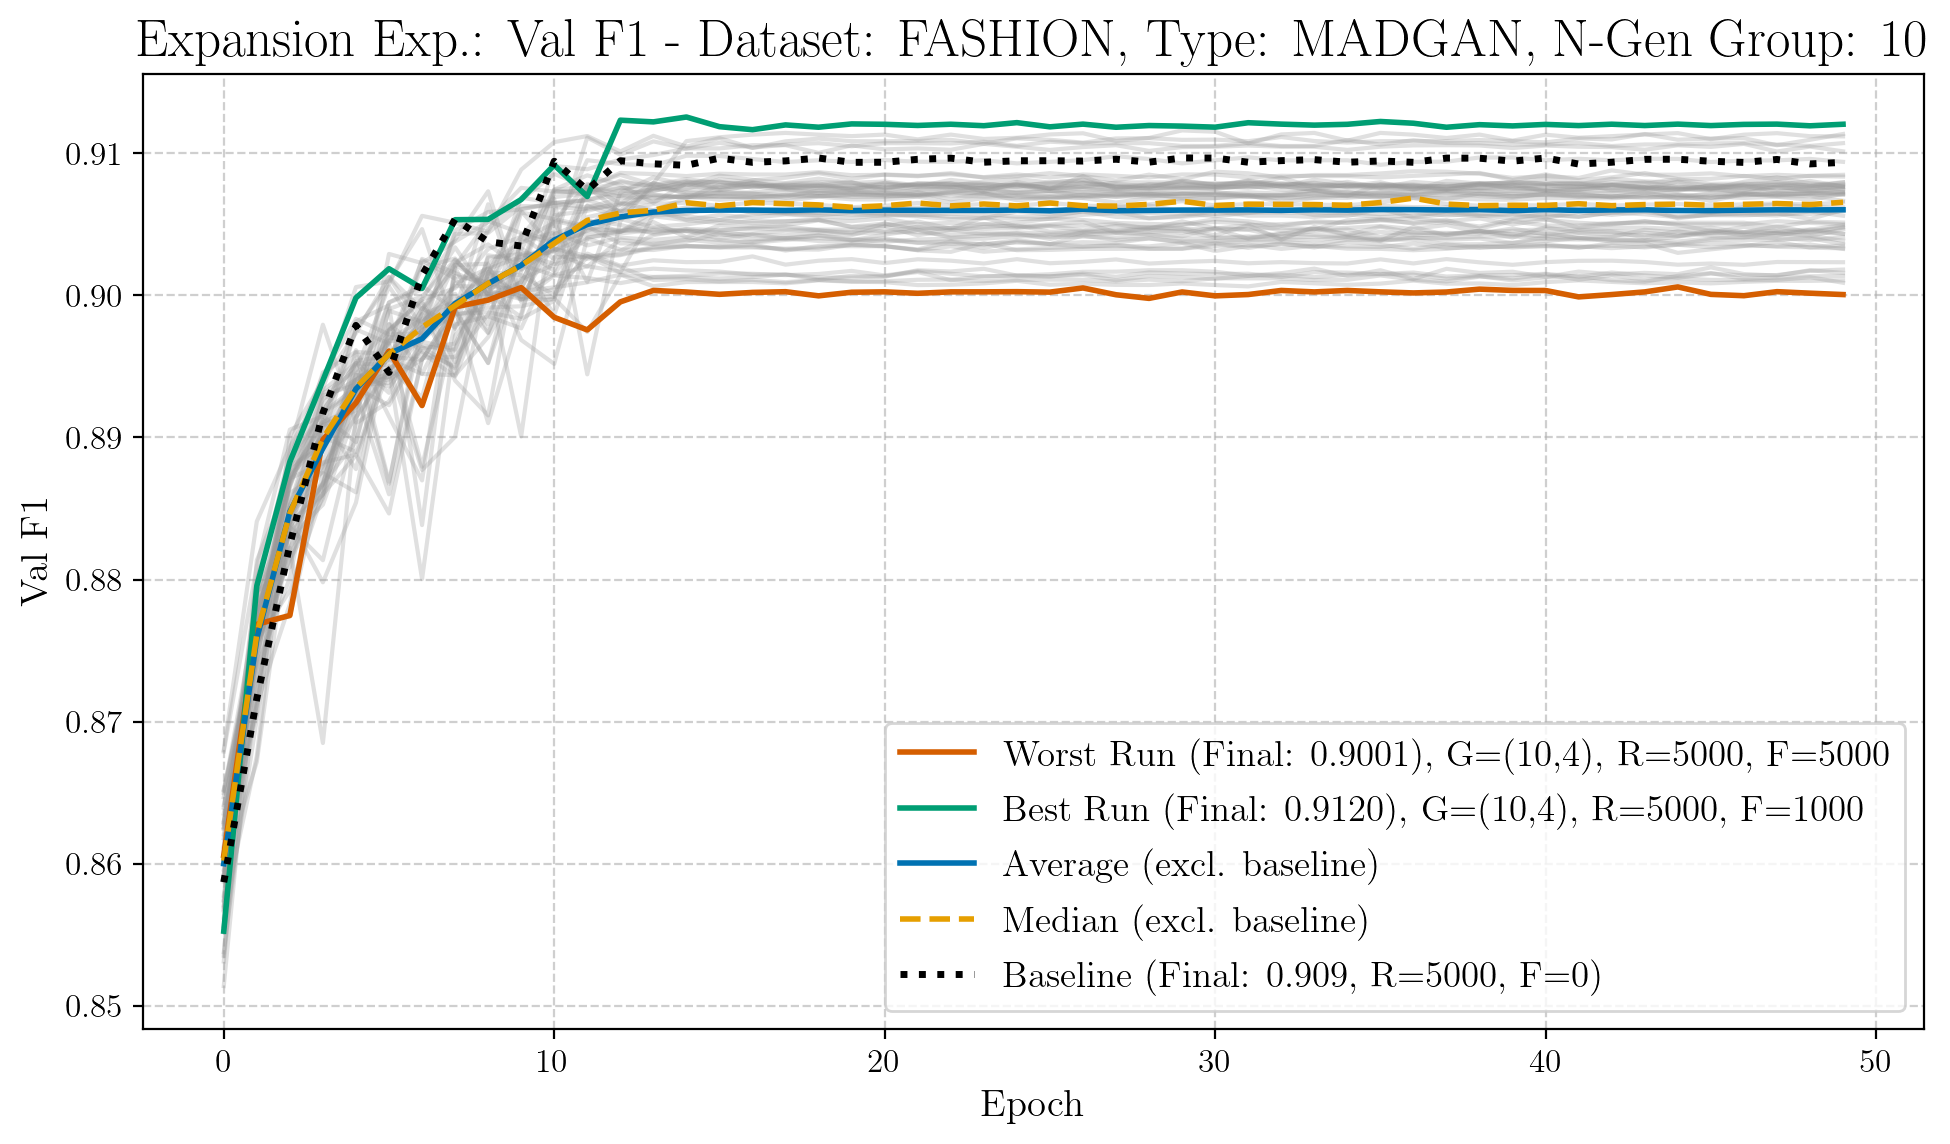
\includegraphics[width=\textwidth]{abb/strat_classifier_performance/FASHION_STRATIFIED_CLASSIFIERS_MADGAN_NEW/expansion_experiments/val_f1_score_MADGAN_FASHION_n_gen_10_all.png}
		\caption{F1 Score on FASHION over 50 epochs. Augmentation tech.: MADGAN (K=10)}
        \label{fig:res_expansion_fashion_cgan_vs_madgan__madgan}
	\end{subfigure}
	\begin{subfigure}{.85\textwidth}
		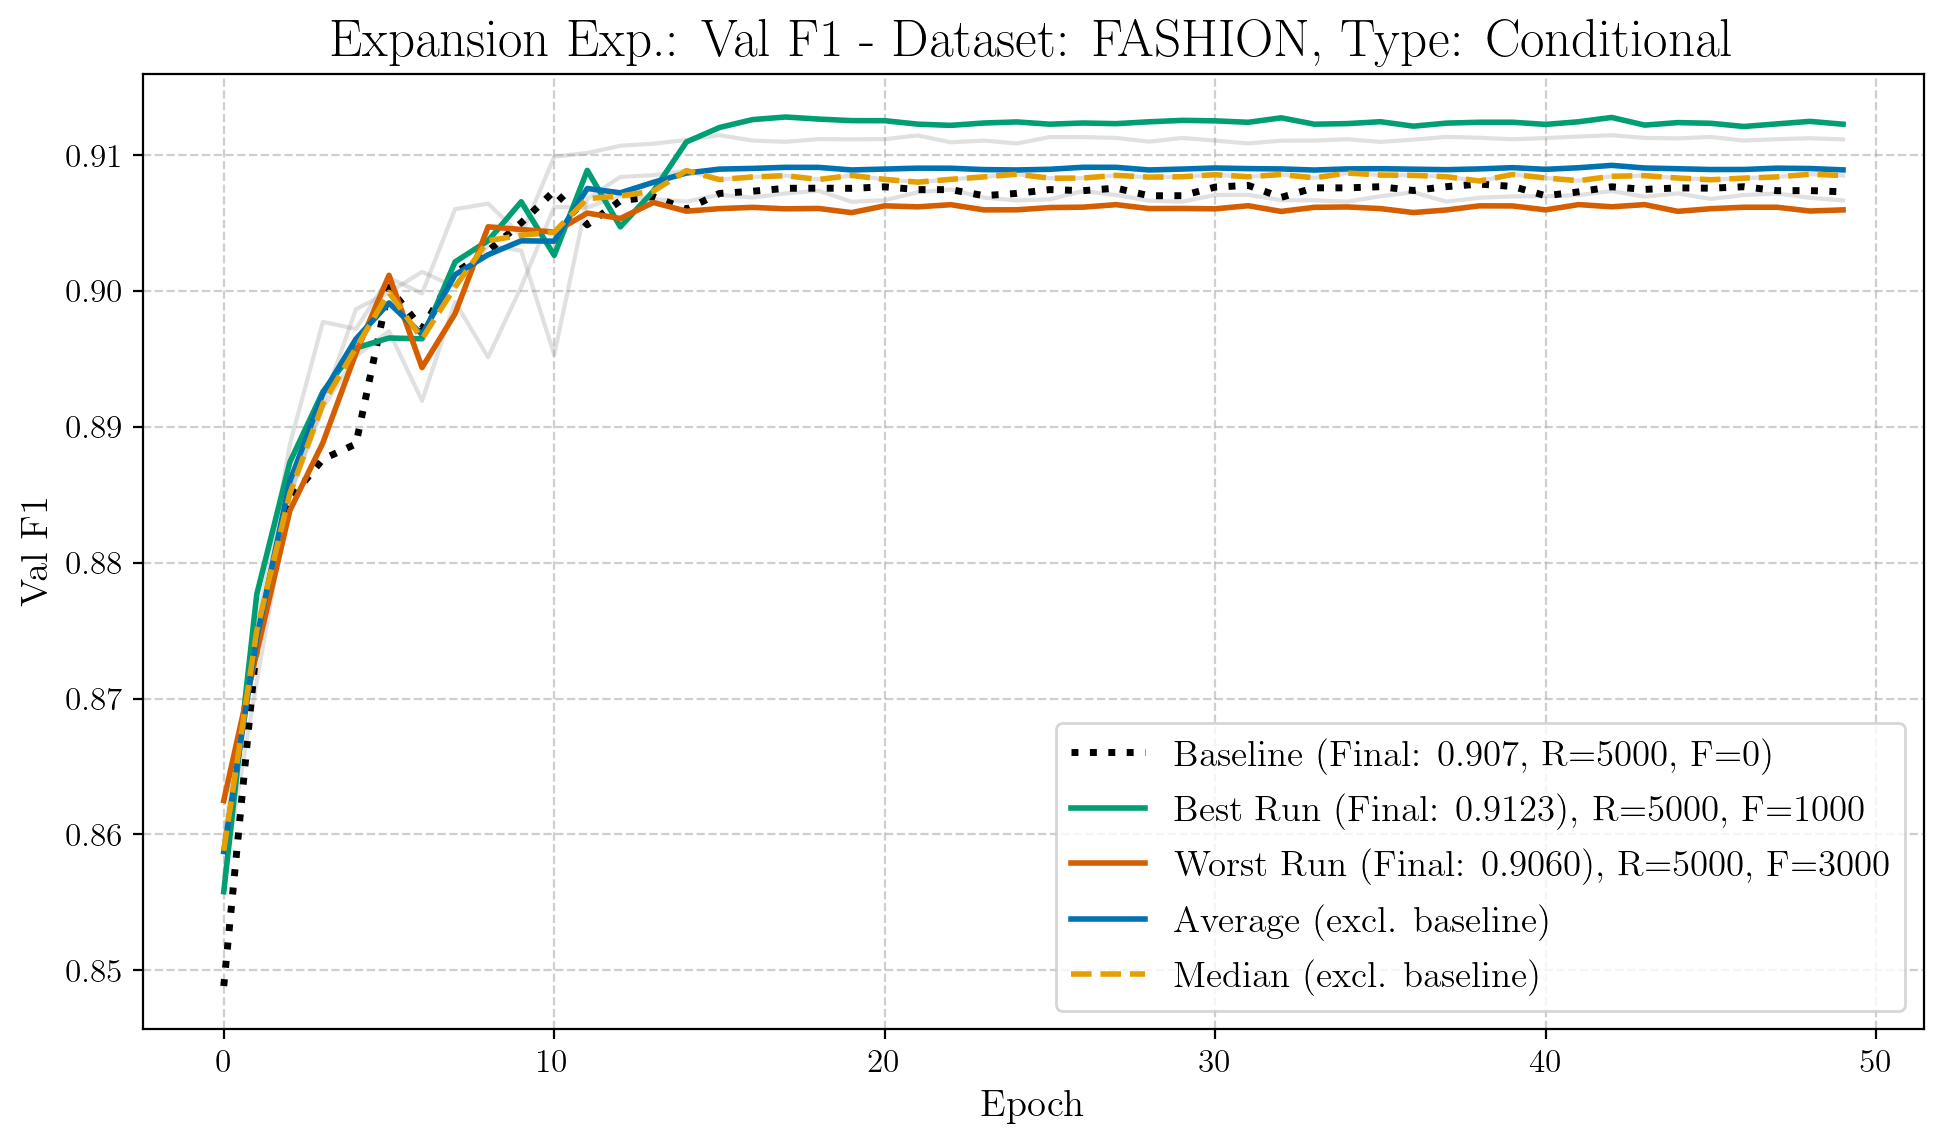
\includegraphics[width=\textwidth]{abb/strat_classifier_performance/FASHION_STRATIFIED_CLASSIFIERS_COND_GAN/expansion_experiments/val_f1_score_['COND']_FASHION_all.png}
		\caption{F1 Score on FASHION over 50 epochs. Augmentation Technique: cGAN}
        \label{fig:res_expansion_fashion_cgan_vs_madgan__cgan}
	\end{subfigure}
%%%%%%%%%%%%%%
\end{figure}

\begin{table}[H]
	\vspace{-1.5em}
	\centering
	\begin{tabular}{|c|c|c|c|}
		\hline
		Run Type & Experiment & Val F1 \\ \hline
		best & \(G_{10, 4}\), R:5000, F:1000 & $0.9120$\\ \hline
		worst & \(G_{10, 4}\), R:5000, F:5000 & $0.9001$\\ \hline
		median & G (K=10) & $0.9066$\\ \hline
		average & (K=10) & $0.9060$
		\\ \hline
	\end{tabular}
    \caption{Final F1 Scores after 50 epochs. Augmentation tech.: MADGAN (K=10)}
        \label{tab:res_expansion_fashion_cgan_vs_madgan__madgan}
\end{table}
\begin{table}[H]
	\centering
	\vspace{-1.5em}
	\begin{tabular}{|c|c|c|c|c|}
		\hline
		Run Type & Experiment & Val F1 \\ \hline
		best & Conditional R:5000, F:1000 & $0.9123$\\ \hline
		worst & Conditional R:5000, F:3000 & $0.9060$\\ \hline
		median & Conditional & $0.9085$\\ \hline
		average & Conditional & $0.9089$
		\\ \hline
	\end{tabular}
    \caption{Final F1 Scores after 50 epochs. Augmentation technique: cGAN}
        \label{tab:res_expansion_fashion_cgan_vs_madgan__cgan}
\end{table}

Both GDA approaches demonstrate effectiveness in the expansion scenario on Fashion-MNIST, achieving high F1 scores that suggest an improvement over a baseline trained on real data alone. The peak performances are very competitive: cGAN achieved a best F1 score of $0.9123$ (when adding 1000 synthetic samples), marginally edging out MADGAN K=10's best F1 score of $0.9120$ (also achieved when adding 1000 synthetic samples from its best generator, \(G_{10,4}\)). These top scores are notably close to the peak performance observed with TDA in previous comparisons.

However, cGAN exhibits slightly better overall consistency and robustness as more synthetic data is added. The average F1 score for cGAN across all expansion levels is $0.9089$, and its median is $0.9085$. These are slightly higher than MADGAN K=10's average ($0.9060$) and median ($0.9066$). More critically, cGAN's worst performance (F1 $0.9060$, when adding 3000 synthetic samples) is substantially better than MADGAN K=10's lowest score (F1 $0.9001$, occurring for generator \(G_{10,4}\) when adding 5000 synthetic samples). This indicates that cGAN's performance degrades less and remains more stable even with larger amounts of synthetic data compared to MADGAN K=10. Consequently, cGAN shows a tighter performance spread (range ~$0.0063$) than MADGAN K=10 (range ~$0.0119$).

In conclusion, for expanding the Fashion-MNIST dataset, both cGAN and MADGAN (K=10) GDA can provide performance benefits, achieving F1 scores competitive with traditional augmentation methods at their peak. However, cGAN demonstrates a slight advantage in overall performance, offering higher average and median scores, and particularly showing greater stability and less degradation when larger volumes of synthetic data are incorporated.

\newpage
\subsubsection[Question 4]{MADGAN GDA vs. cMADGAN GDA Performance}      \label{exp_results_ans_q4}
Ultimately, the final direct comparison sets MADGAN and the conditional adaptation cMADGAN side-by-side. As established before, the best selection of MADGAN experiments (K=10 for Replacement-, K=7 for Expansion scenario on MNIST and K=7 for Replacement-, K=10 for Expansion scenario on Fashion-MNIST) is directly compared against the best performing setting of cMADGAN. Orienting on the afore comparison against MADGAN vs. DCGAN/cGAN (\ref{exp_results_ans_q3}). Other references to cMADGAN experiments from the appendix are mentioned were reasonable. 

% TODO: preamble the results of the following experiments

\newpage

\noindent\textbf{Replacement Experiment, Dataset: MNIST}
\begin{figure}[H]
	\centering
	\begin{subfigure}{.85\textwidth}
		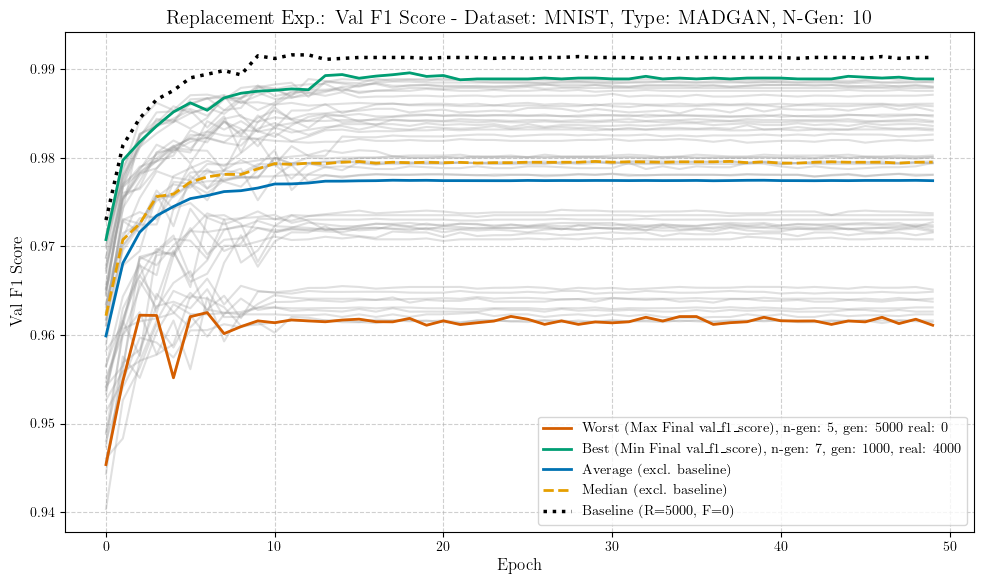
\includegraphics[width=\textwidth]{abb/strat_classifier_performance/MNIST_STRATIFIED_CLASSIFIERS_MADGAN_NEW/replacement_experiments/val_f1_score_MADGAN_MNIST_n_gen_10_all.png}
		\caption{F1 Score on MNIST over 50 epochs. Augmentation technique: MADGAN (K=10)}
        \label{fig:res_replacement_mnist_cmadgan_vs_madgan__madgan}
	\end{subfigure}
	\begin{subfigure}{.85\textwidth}
		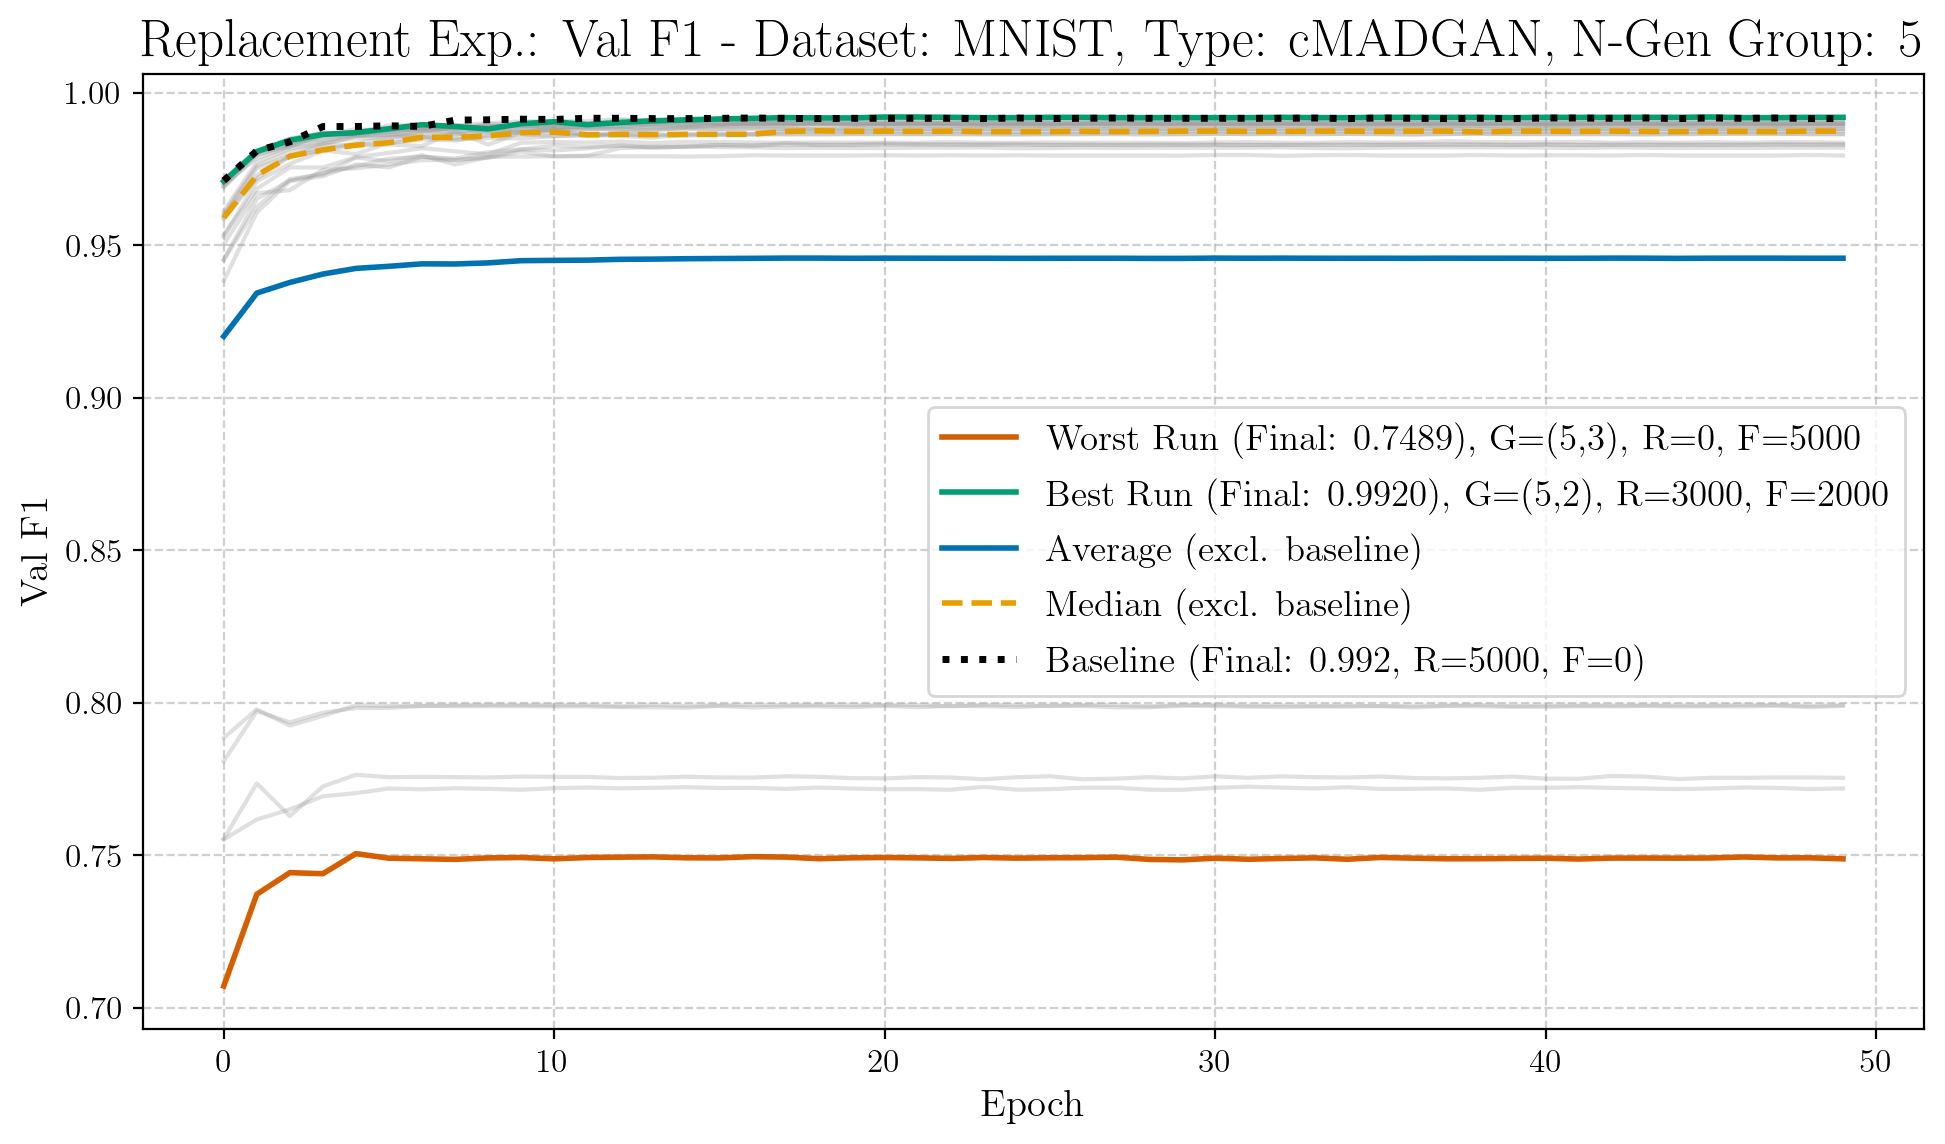
\includegraphics[width=\textwidth]{abb/strat_classifier_performance/MNIST_STRATIFIED_CLASSIFIERS_cMADGAN_NEW/replacement_experiments/val_f1_score_cMADGAN_MNIST_n_gen_5_all.png}
		\caption{F1 Score on MNIST over 50 epochs. Augmentation technique: cMADGAN (K=5)}
        \label{fig:res_replacement_mnist_cmadgan_vs_madgan__cmadgan}
	\end{subfigure}
%%%%%%%%%%%%%%
\end{figure}

\begin{table}[H]
	\vspace{-1.5em}
	\centering
	\begin{tabular}{|c|c|c|c|}
		\hline
		Run Type & Experiment & Val F1 \\ \hline
		best & \(G_{10, 7}\), R:4000, F:1000 & $0.9889$\\ \hline
		worst & \(G_{10, 5}\), R:0, F:5000 & $0.9611$\\ \hline
		median & G (K=10) & $0.9795$\\ \hline
		average & G (K=10) & $0.9774$
		\\ \hline
	\end{tabular}
    \caption{Final F1 Scores after 50 epochs. Augmentation technique: MADGAN (K=10)}
        \label{tab:res_replacement_mnist_cmadgan_vs_madgan__madgan}
\end{table}
\begin{table}[H]
	\centering
	\vspace{-1.5em}
	\begin{tabular}{|c|c|c|c|c|}
		\hline
		Run Type & Experiment & Val F1 \\ \hline
		best & \(G_{5, 2}\), R:3000, F:2000 & $0.9920$\\ \hline
		worst & \(G_{5, 3}\), R:0, F:5000 & $0.7489$\\ \hline
		median & G (K=5) & $0.9874$\\ \hline
		average & G (K=5) & $0.9458$
		\\ \hline
	\end{tabular}
    \caption{Final F1 Scores after 50 epochs. Augmentation technique: cMADGAN (K=5)}
        \label{tab:res_replacement_mnist_cmadgan_vs_madgan__cmadgan}
\end{table}
The comparison reveals a fascinating trade-off between peak performance potential and consistency. The cMADGAN (K=5) model achieved the highest individual F1 score in this set of experiments, reaching $0.9920$ (with generator \(G_{5,2}\) when replacing 2000 real samples with 2000 synthetic ones per class from the R:5000/F:0 baseline). This peak performance is notably high, surpassing the best score from MADGAN K=10 ($0.9889$) and even rivaling the top scores seen with Traditional Data Augmentation (TDA) in previous comparisons. This suggests that individual generators within the cMADGAN K=5 framework can produce highly effective synthetic data for replacement.

However, cMADGAN K=5 exhibits extreme variability. Its worst performing run (generator \(G_{5,3}\) when using only synthetic data, R:0, F:5000) resulted in a drastically low F1 score of $0.7489$. This drop for at least one of its generators signifies a lack of reliability. It is to note, that four other generators resulted with similar lower scores, between $0.75$ and $0.8$. In contrast, MADGAN K=10, while not reaching the same peak as cMADGAN K=5, demonstrated much greater consistency. Its most adverse F1 score was $0.9611$, indicating that even its poorest performing generator at full replacement maintained a high level of performance.

This difference in variability influences the average and median scores. MADGAN K=10 achieved a substantially better average F1 score ($0.9774$) compared to cMADGAN K=5 ($0.9458$), as the latter's average was significantly pulled down by its low outlier(s). Conversely, cMADGAN K=5 reported a higher median F1 score ($0.9874$) than MADGAN K=10 ($0.9795$), suggesting that the typical performance of a cMADGAN K=5 generator (excluding the worst cases) is very strong and even surpasses the typical MADGAN K=10 generator. The overall performance spread for cMADGAN K=5 (range ~$0.2431$) is vastly larger than that of MADGAN K=10 (range ~$0.0278$).

To conclude, for the replacement task on MNIST, cMADGAN (K=5) offers the potential for superior peak GDA performance from its best generators, achieving results competitive with the best augmentation methods. However, it suffers from significant inconsistency, with some generators producing very poor quality synthetic data leading to a low average performance. MADGAN (K=10) provides more reliable and stable GDA performance, with a better average F1 score and a much more dependable weakest performing outcome, though its peak performance is slightly lower than the best of cMADGAN (K=5). Overall, the MADGANs reliability, proved itself, almost regardless of the number of generators used \ref{app_strat_class_performance_madgan_mnist}. cMADGAN, on the other hand, showed to be less reliable overall, consistently resulting in a couple of bad generators, in terms of their augmentation performance \ref{app_strat_class_performance_cmadgan_mnist}.


\newpage
\noindent\textbf{Expansion Experiment, Dataset: MNIST}
\begin{figure}[H]
	\centering
	\begin{subfigure}{.85\textwidth}
		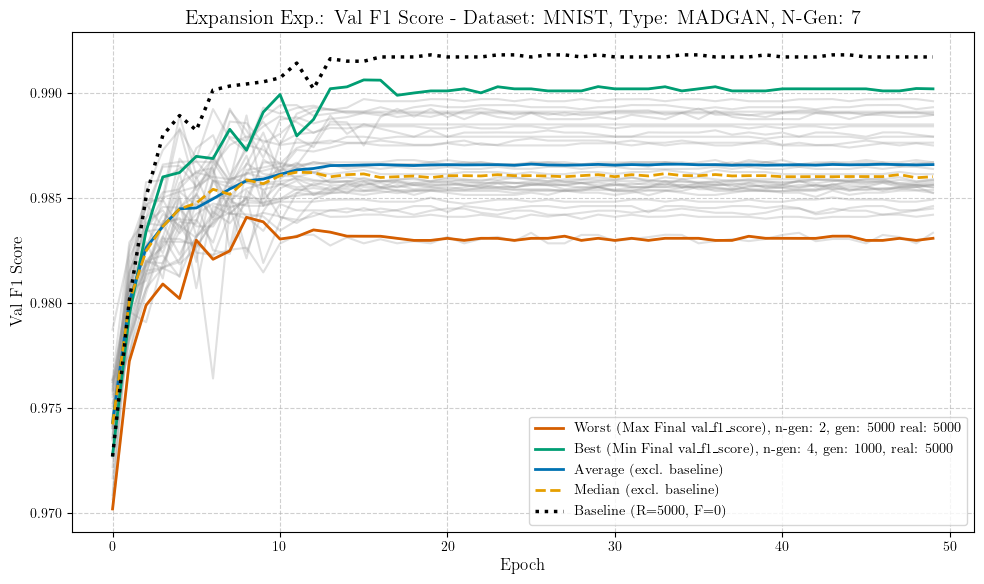
\includegraphics[width=\textwidth]{abb/strat_classifier_performance/MNIST_STRATIFIED_CLASSIFIERS_MADGAN_NEW/expansion_experiments/val_f1_score_MADGAN_MNIST_n_gen_7_all.png}
		\caption{F1 Score on MNIST over 50 epochs. Augmentation tech.: MADGAN (K=7)}
        \label{fig:res_expansion_mnist_cmadgan_vs_madgan__madgan}
	\end{subfigure}
	\begin{subfigure}{.85\textwidth}
		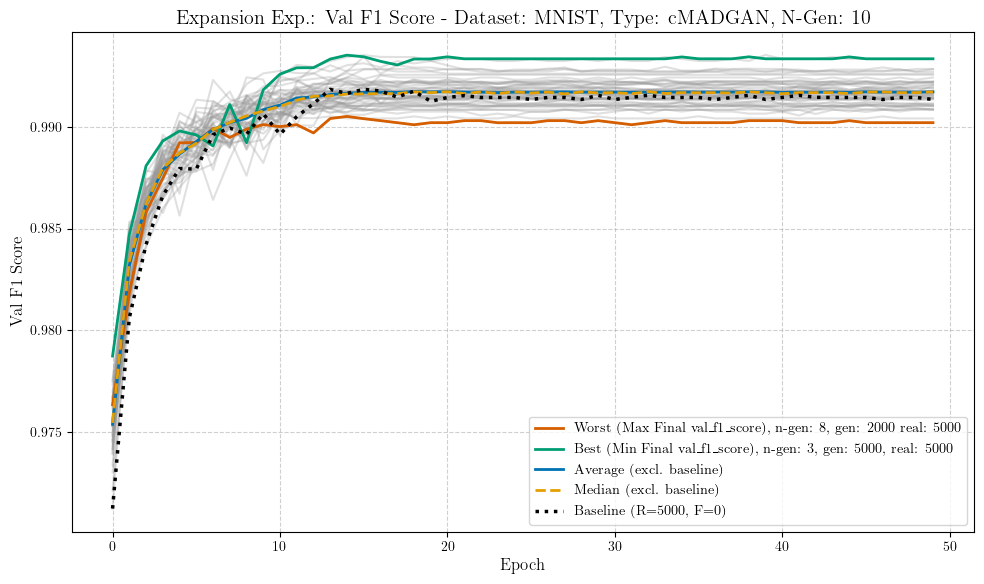
\includegraphics[width=\textwidth]{abb/strat_classifier_performance/MNIST_STRATIFIED_CLASSIFIERS_cMADGAN_NEW/expansion_experiments/val_f1_score_cMADGAN_MNIST_n_gen_10_all.png}
		\caption{F1 Score on MNIST over 50 epochs. Augmentation tech.: cMADGAN (K=10)}
        \label{fig:res_expansion_mnist_cmadgan_vs_madgan__cmadgan}
	\end{subfigure}
%%%%%%%%%%%%%%
\end{figure}

\begin{table}[H]
	\vspace{-1.5em}
	\centering
	\begin{tabular}{|c|c|c|c|}
		\hline
		Run Type & Experiment & Val F1 \\ \hline
		best & \(G_{7, 4}\), R:5000, F:1000 & $0.9902$\\ \hline
		worst & \(G_{7, 2}\), R:5000, F:5000 & $0.9831$\\ \hline
		median & G (K=7) & $0.9860$\\ \hline
		average & G (K=7) & $0.9866$
		\\ \hline
	\end{tabular}
    \caption{Final F1 Scores after 50 epochs. Augmentation tech.: MADGAN (K=10)}
        \label{tab:res_expansion_mnist_cmadgan_vs_madgan__madgan}
\end{table}
\begin{table}[H]
	\centering
	\vspace{-1.5em}
	\begin{tabular}{|c|c|c|c|c|}
		\hline
		Run Type & Experiment & Val F1 \\ \hline
		best & \(G_{10, 3}\), R:5000, F:5000 & $0.9933$\\ \hline
		worst & \(G_{10, 8}\), R:5000, F:2000 & $0.9902$\\ \hline
		median & G (K=10) & $0.9917$\\ \hline
		average & G (K=10) & $0.9917$
		\\ \hline
	\end{tabular}
    \caption{Final F1 Scores after 50 epochs. Augmentation tech.: cMADGAN (K=10)}
        \label{tab:res_expansion_mnist_cmadgan_vs_madgan__cmadgan}
\end{table}

The results compellingly demonstrate the superiority of cMADGAN (K=10) over MADGAN (K=7) for data expansion on MNIST. Across all summary statistics, cMADGAN (K=10) achieves markedly better and more consistent F1 scores.

Specifically, the best F1 score attained by cMADGAN (K=10) is $0.9933$ (generator \(G_{10,3}\) when adding 5000 synthetic samples), which is not only significantly higher than MADGAN K=7's best of $0.9902$ but is also highly competitive with the peak performance observed using Traditional Data Augmentation (TDA, previously around $0.9938$). Remarkably, this peak for cMADGAN K=10 occurs at the maximum level of data expansion (F:5000), indicating a strong positive contribution from the synthetic data.

The robustness of cMADGAN K=10 is further highlighted by its weakest performance. Its lowest F1 score across all its generators and expansion ratios is $0.9902$. Strikingly, this worst score for cMADGAN K=10 is identical to the best score achieved by MADGAN K=7. In contrast, MADGAN K=7's performance drops to $0.9831$ in its pessimistic scenario.

Consequently, the average ($0.9917$) and median ($0.9917$) F1 scores for cMADGAN K=10 are substantially higher than those for MADGAN K=7 (average $0.9866$, median $0.9860$). Moreover, cMADGAN K=10 exhibits a much tighter performance cluster, with a very small spread between its best and worst scores (range ~$0.0031$), indicating high consistency across its generators and different levels of augmentation. This contrasts with MADGAN K=7's larger spread (range ~$0.0071$).

In conclusion, for the MNIST expansion task, cMADGAN (K=10) GDA proves to be a significantly more effective and reliable augmentation technique than MADGAN (K=7) GDA. It not only achieves higher peak performance that rivals traditional methods but also maintains excellent scores with minimal variability even when large volumes of synthetic data are introduced, showcasing its strong potential for enhancing classifier training. Graphs in the appendix further strengthen the claims made \ref{app_strat_class_performance_cmadgan_mnist}.


\newpage
\noindent\textbf{Replacement Experiment, Dataset: Fashion-MNIST}
\begin{figure}[H]
	\centering
	\begin{subfigure}{.85\textwidth}
		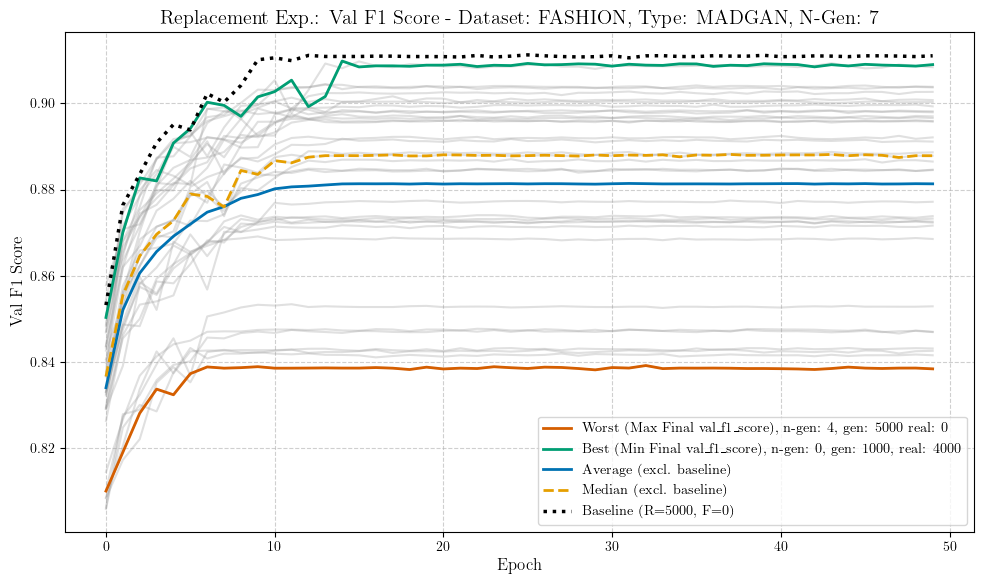
\includegraphics[width=\textwidth]{abb/strat_classifier_performance/FASHION_STRATIFIED_CLASSIFIERS_MADGAN_NEW/replacement_experiments/val_f1_score_MADGAN_FASHION_n_gen_7_all.png}
		\caption{F1 Score on FASHION over 50 epochs. Augmentation tech.: MADGAN (K=7)}
        \label{fig:res_replacement_fashion_cmadgan_vs_madgan__madgan}
	\end{subfigure}
	\begin{subfigure}{.85\textwidth}
		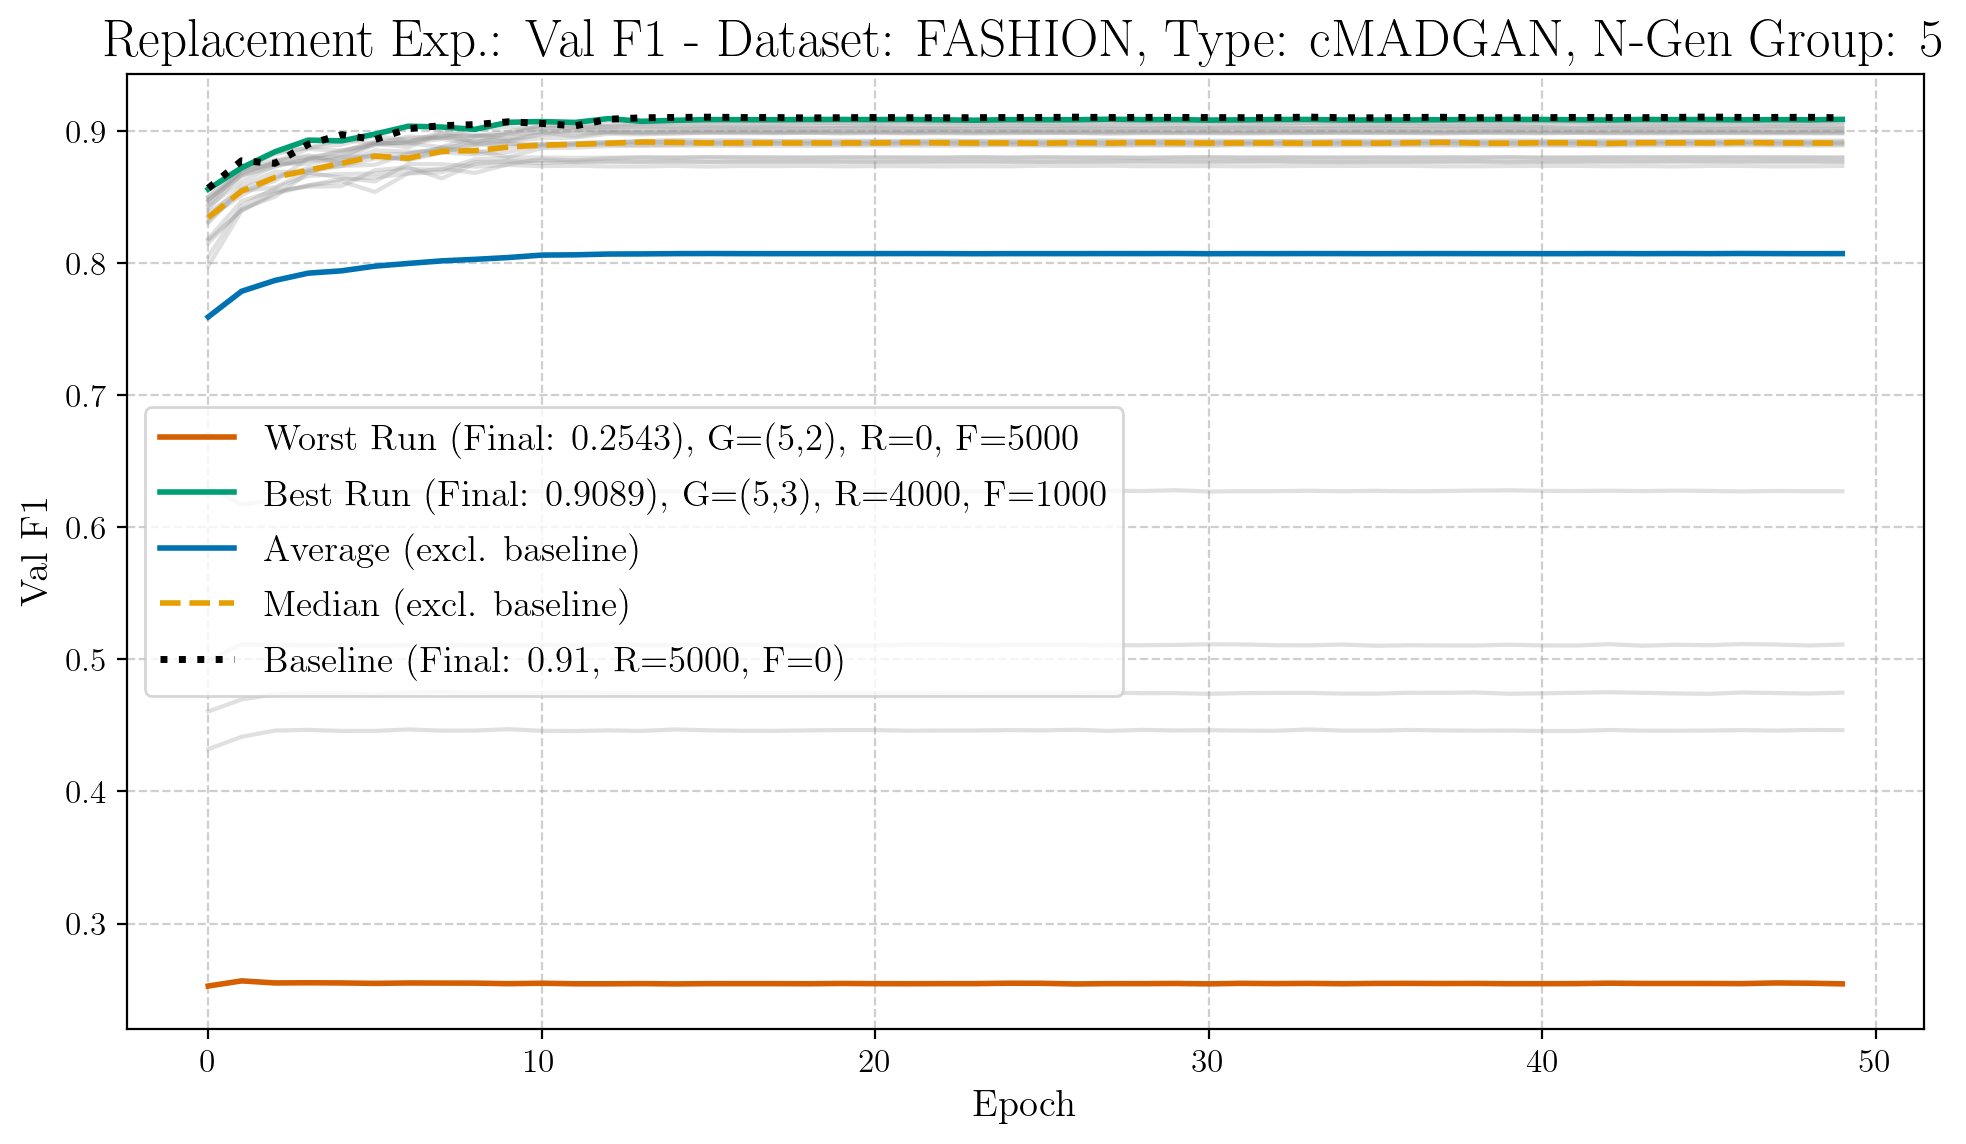
\includegraphics[width=\textwidth]{abb/strat_classifier_performance/FASHION_STRATIFIED_CLASSIFIERS_cMADGAN_NEW/replacement_experiments/val_f1_score_cMADGAN_FASHION_n_gen_5_all.png}
		\caption{F1 Score on FASHION over 50 epochs. Augmentation tech.: cMADGAN (K=5)}
        \label{fig:res_replacement_fashion_cmadgan_vs_madgan__cmadgan}
	\end{subfigure}
%%%%%%%%%%%%%%
\end{figure}

\begin{table}[H]
	\vspace{-1.5em}
	\centering
	\begin{tabular}{|c|c|c|c|}
		\hline
		Run Type & Experiment & Val F1 \\ \hline
		best & \(G_{7, 0}\), R:4000, F:1000 & $0.9090$\\ \hline
		worst & \(G_{7, 4}\), R:0, F:5000 & $0.8384$\\ \hline
		median & G (K=7) & $0.8879$\\ \hline
		average & G (K=7) & $0.8813$
		\\ \hline
	\end{tabular}
    \caption{Final F1 Scores after 50 epochs. Augmentation tech.: MADGAN (K=7)}
        \label{tab:res_replacement_fashion_cmadgan_vs_madgan__madgan}
\end{table}
\begin{table}[H]
	\centering
	\vspace{-1.5em}
	\begin{tabular}{|c|c|c|c|c|}
		\hline
		Run Type & Experiment & Val F1 \\ \hline
		best & \(G_{5, 3}\), R:4000, F:1000 & $0.9089$\\ \hline
		worst & \(G_{5, 2}\), R:0, F:5000 & $0.2543$\\ \hline
		median & G (K=5) & $0.8909$\\ \hline
		average & G (K=5) & $0.8072$
		\\ \hline
	\end{tabular}
    \caption{Final F1 Scores after 50 epochs. Augmentation tech.: cMADGAN (K=5)}
        \label{tab:res_replacement_fashion_cmadgan_vs_madgan__cmadgan}
\end{table}

Both multi-generator approaches demonstrate the capability to achieve high peak F1 scores when a limited amount of real data is replaced. cMADGAN (K=5) achieved a slightly lower best F1 score of $0.9089$ (generator \(G_{5,3}\) with R:4000, F:1000), marginally falling short of MADGAN K=7's best of $0.9090$ (generator \(G_{7,0}\) with R:4000, F:1000). Notably, these peak performances from both models are competitive with, and even slightly exceed, the best scores previously observed with Traditional Data Augmentation (TDA) on this dataset.

However, this high peak potential is starkly contrasted by extreme inconsistency and poor performance when relying heavily on synthetic data, particularly when all real data is substituted. cMADGAN (K=5) exhibited the lowest and lest robust F1 score, dropping to a critically low $0.2543$ (generator \(G_{5,2}\) with R:0, F:5000). While MADGAN K=7's lowest score ($0.8384$ from generator \(G_{7,4}\) with R:0, F:5000) was also degraded, it remained significantly above cMADGAN K=5's absolute floor.

These extreme low scores significantly impact the overall assessment. Despite its lower absolute worst score, cMADGAN (K=5) managed a slightly higher median F1 score ($0.8909$) compared to MADGAN K=7 ($0.8879$). This suggests that, aside from its most extreme outliers, the bulk of cMADGAN K=5's generator/ratio combinations might perform marginally better than those of MADGAN K=7. Conversely, MADGAN K=7 shows a slightly better average F1 score ($0.8813$) than cMADGAN K=5 ($0.8072$), indicating its typical performance, discounting the severe negative outliers from both, might be marginally more consistent. Both models display very large performance spreads, with cMADGAN K=5 having a significantly wider range due to its lower floor.

Taken together, for the Fashion-MNIST replacement task, both MADGAN (K=7) and cMADGAN (K=5) can produce synthetic data from their best generators that lead to excellent, TDA-competitive classifier performance with limited replacement. Nonetheless, both frameworks suffer from extreme variability, cMADGAN more so than MADGAN. Both contain individual generators that produce very poor-quality data for this task, leading to unusable classifiers when real data is fully replaced. While cMADGAN K=5 achieved a slightly higher median, its weakest result was more severe, making both models unreliable for extensive data replacement compared to more stable traditional methods, despite their promising best-case results. Ultimately, the results show, that the presented GDA methods must be strictly controlled and carefully monitored to use them. Acting upon average results might mask single bad performances, at least in the replacement scenarios. 



\newpage
\noindent\textbf{Expansion Experiment, Dataset: Fashion-MNIST}
\begin{figure}[H]
	\centering
	\begin{subfigure}{.85\textwidth}
		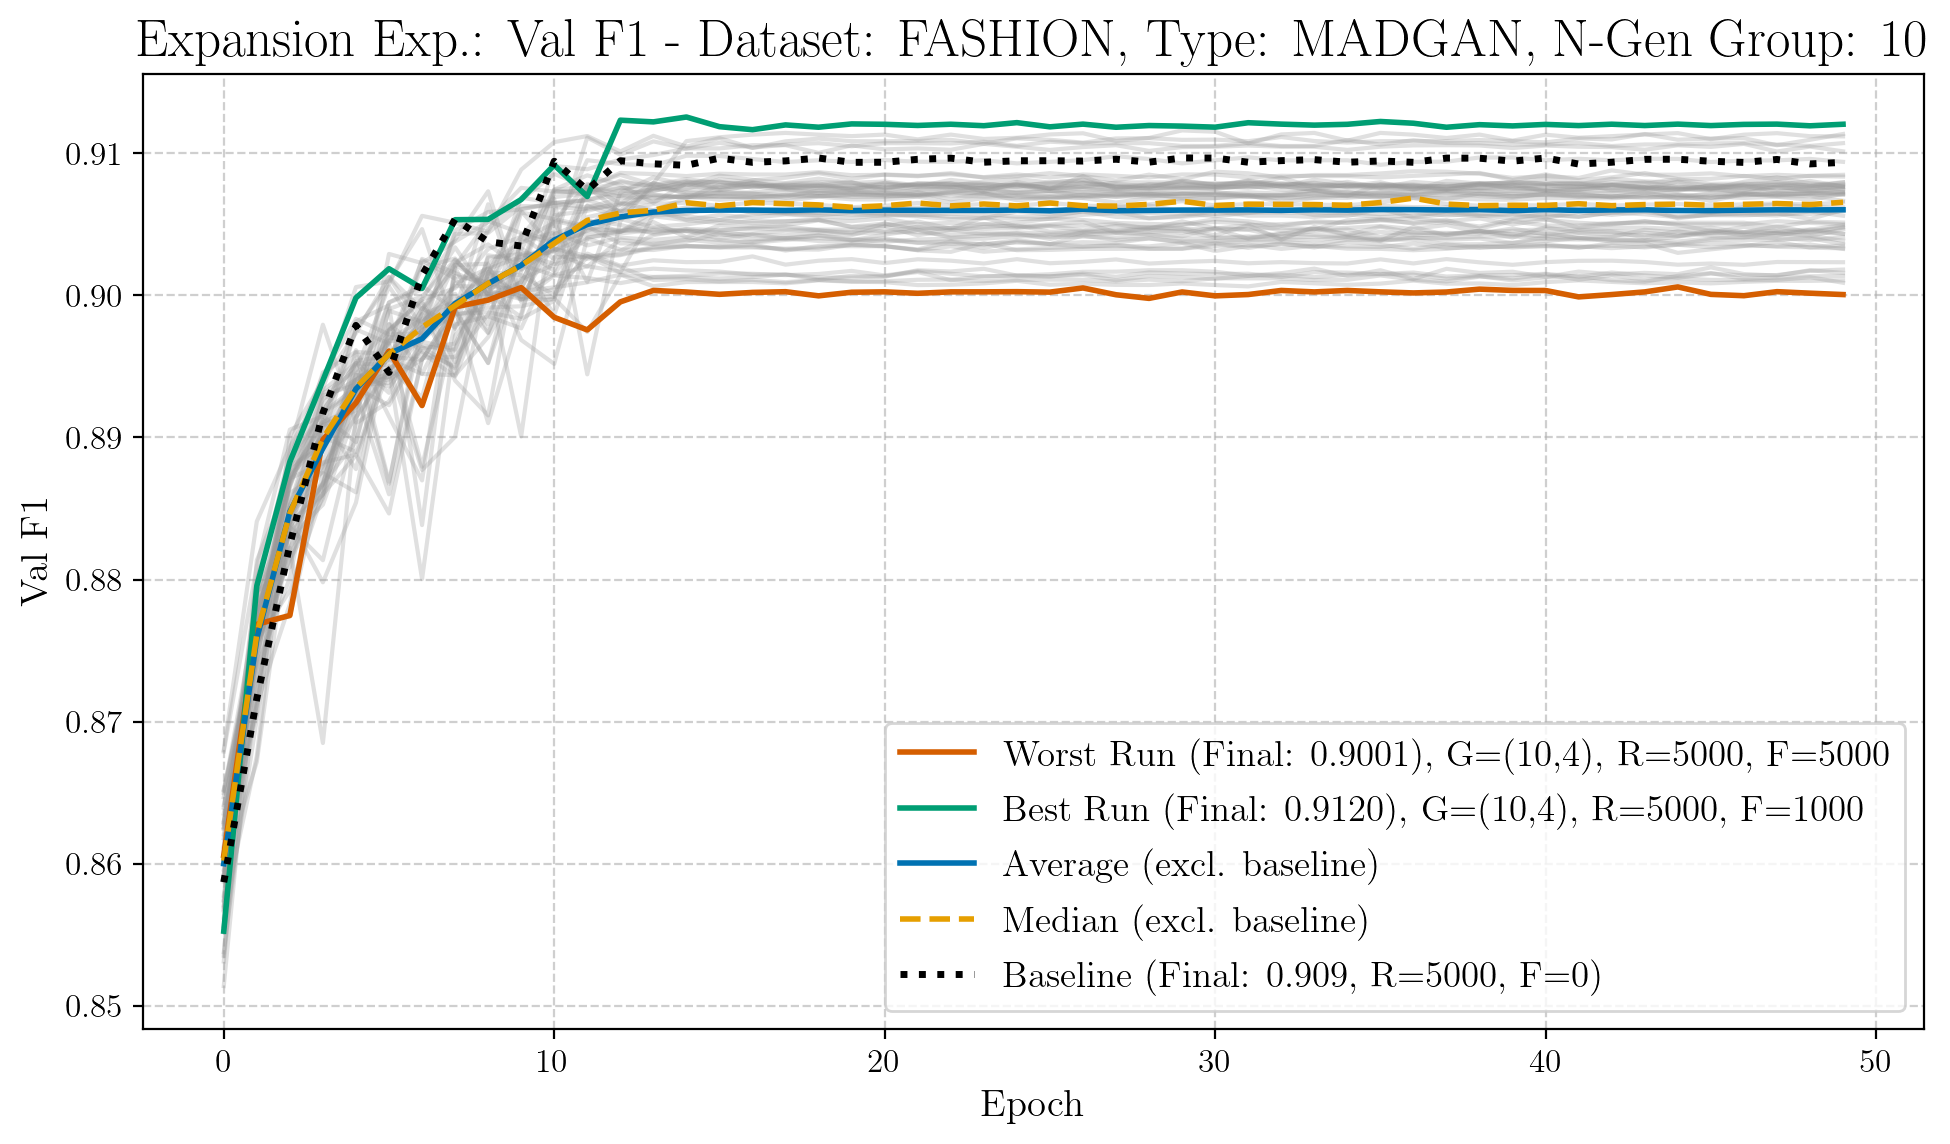
\includegraphics[width=\textwidth]{abb/strat_classifier_performance/FASHION_STRATIFIED_CLASSIFIERS_MADGAN_NEW/expansion_experiments/val_f1_score_MADGAN_FASHION_n_gen_10_all.png}
		\caption{F1 Score on FASHION over 50 epochs. Augmentation tech.: MADGAN (K=10)}
        \label{fig:res_expansion_fashion_cmadgan_vs_madgan__madgan}
	\end{subfigure}
	\begin{subfigure}{.85\textwidth}
		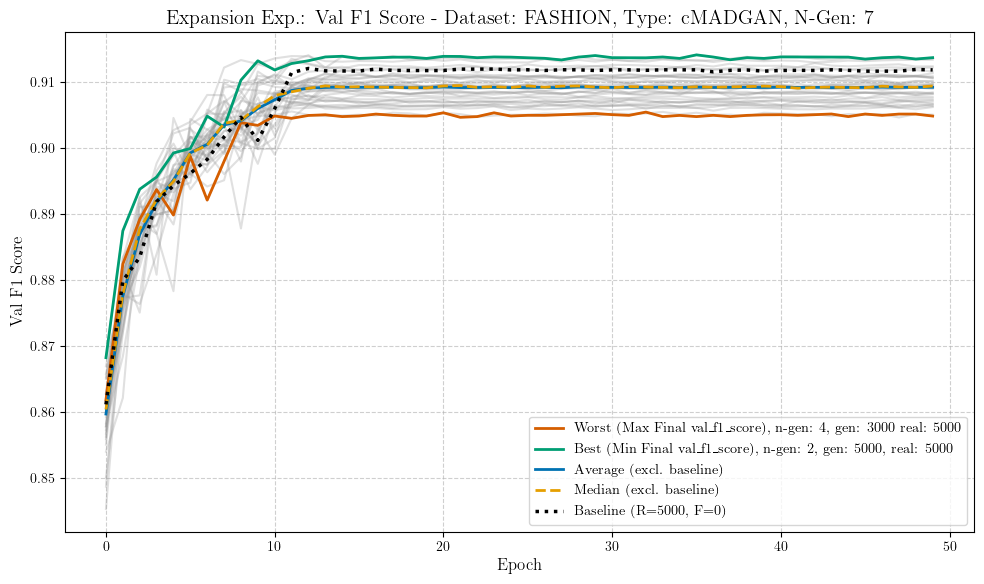
\includegraphics[width=\textwidth]{abb/strat_classifier_performance/FASHION_STRATIFIED_CLASSIFIERS_cMADGAN_NEW/expansion_experiments/val_f1_score_cMADGAN_FASHION_n_gen_7_all.png}
		\caption{F1 Score on FASHION over 50 epochs. Augmentation tech.: cMADGAN (K=7)}
        \label{fig:res_expansion_fashion_cmadgan_vs_madgan__cmadgan}
	\end{subfigure}
%%%%%%%%%%%%%%
\end{figure}

\begin{table}[H]
	\vspace{-1.5em}
	\centering
	\begin{tabular}{|c|c|c|c|}
		\hline
		Run Type & Experiment & Val F1 \\ \hline
		best & \(G_{10, 4}\), R:5000, F:1000 & $0.9120$\\ \hline
		worst & \(G_{10, 4}\), R:5000, F:5000 & $0.9001$\\ \hline
		median & G (K=10) & $0.9066$\\ \hline
		average & (K=10) & $0.9060$
		\\ \hline
	\end{tabular}
    \caption{Final F1 Scores after 50 epochs. Augmentation tech.: MADGAN (K=10)}
        \label{tab:res_expansion_fashion_cmadgan_vs_madgan__madgan}
\end{table}
\begin{table}[H]
	\centering
	\vspace{-1.5em}
	\begin{tabular}{|c|c|c|c|c|}
		\hline
		Run Type & Experiment & Val F1 \\ \hline
		best & \(G_{7, 2}\), R:5000, F:5000 & $0.9138$\\ \hline
		worst & \(G_{7, 4}\), R:5000, F:3000 & $0.9049$\\ \hline
		median & G (K=7) & $0.9095$\\ \hline
		average & G (K=7) & $0.9093$
		\\ \hline
	\end{tabular}
    \caption{Final F1 Scores after 50 epochs. Augmentation tech.: cMADGAN (K=7)}
        \label{tab:res_expansion_fashion_cmadgan_vs_madgan__cmadgan}
\end{table}

The results are indicating a clear advantage for cMADGAN (K=7) over MADGAN (K=10) in the expansion scenario on Fashion-MNIST. Here, cMADGAN (K=7) is demonstrating superior performance across all metrics aggregated in the table \ref{tab:res_expansion_fashion_cmadgan_vs_madgan__cmadgan}, compared to \ref{tab:res_expansion_fashion_cmadgan_vs_madgan__madgan}.

cMADGAN (K=7) achieved a remarkable peak F1 score of $0.9138$ (with generator \(G_{7,2}\) when adding the maximum of 5000 synthetic samples per class). This is the highest F1 score recorded among all GDA methods on Fashion-MNIST in these expansion experiments and is highly competitive with the best scores from Traditional Data Augmentation (TDA, previously $0.9129$). The fact that this peak occurs at maximum data expansion is particularly noteworthy. Furthermore, cMADGAN K=7's pessimistic F1 score ($0.9049$) is impressively high, indicating strong performance even from its least effective generator/ratio combination.

In comparison, MADGAN (K=10) achieved a best F1 score of $0.9120$ (generator \(G_{10,4}\) with R:5000, F:1000), slightly below cMADGAN K=7's peak. More significantly, MADGAN K=10's minimal F1 score dropped to $0.9001$, which, while still good, is notably lower than cMADGAN K=7's lowest result.

This superiority of cMADGAN K=7 is further reflected in its average ($0.9093$) and median ($0.9095$) F1 scores, both of which are higher than MADGAN K=10's average ($0.9060$) and median ($0.9066$). Additionally, cMADGAN (K=7) exhibited a tighter performance distribution, with a smaller spread between its best and worst scores ($0.0089$) compared to MADGAN K=10 ($0.0119$), signifying greater consistency.

In conclusion, for the Fashion-MNIST expansion task, cMADGAN (K=7) emerges as the more effective and reliable GDA technique compared to MADGAN (K=10). It not only achieves a higher peak F1 score that rivals TDA but also delivers better average performance and greater robustness, maintaining strong results. This is especially true when substantially expanding the dataset with generated samples. The MADGAN architecture classifiers, on the other hand, performed worst with the highest amount of augmented samples.

\subsubsection[Question 5]{Effect of increasing the Generators}            \label{exp_results_ans_q5}
The following paragraphs conclude the experimental section and answers question 5 (\ref{exp_results_research_questions}). Above experiments are used to conclude the effect of adjusting \textbf{K} (the number of generators in multi-agent GAN architectures). First, the sections focus the MADGAN- and secondly the cMADGAN architecture. To answer this question, all experiments, including those present in the appendix are taken into consideration.

% labels for fid is scores:
% \label{exp_ans_q1_mnsit_fid_is}, \label{exp_ans_q1_fmnsit_fid_is}c

\noindent\textbf{MADGAN}
Across the datasets (MNIST, Fashion-MNIST), increasing K positively correlated with an increase of image quality and diversity, judged by the average FID and IS. Especially for the Fashion-MNIST dataset, the MADGAN with $K=10$ performed the best. This setting achieved the lowest FID and the highest IS, excluding the baseline \ref{tab:exp_fashionmnist_fid_is}. The results on MNIST, however, show that this trend does not fully generalize. The MADGAN with $K=10$ does result in the lowest FID. The IS, on the other hand, is the third highest from four (\ref{tab:exp_mnist_fid_is}). Analyzing the scores for the single generator evaluations, the lowest FID score results from the ninth generator from the $K=10$ experiment. The highest IS occurred in the setting with $K=7$ (\ref{tab:app_madgan_mnist_fid_is}). For MNIST the lowest FID and highest IS are created by the generator \(G_{10,4}\).

Taking the Replacement and Expansion scenarios into consideration, the MADGAN architecture performed best with a value, close to the number of classes in the dataset. For the Replacement scenario on MNIST, $K=10$ and for the Expansion scenario $K=7$ achieved the highest F1 scores. In accordance to these results, the outcome on Fashion-MNIST was the same, with $K=7$ and $K=10$ performing best on the two scenarios respectively.

Overall, it can be concluded that the increase of $K$ generally improved the performance of the MADGANs, especially for the Fashion-MNIST dataset. The effect is, however, less consistent on the MNIST dataset. \\

\noindent\textbf{cMADGAN}
The same cannot be said about the cMADGAN architecture. In fact, the opposite is the case here. On MNIST, the best FID and IS can be found with $K=3$. Here, the lowest FID score is achieved by generator \(G_{3,2}\), with $22.753$ and the highest IS achieved by generator \(G_{3,0}\), with $2.494$ (\ref{tab:cmadgan_mnist_fid_is}). The averaged performance of the architecture with growing $K$ showed a monotonic increase of the FID, pointing at a negative correlation between the number of generators and the quality of the generated images, judged by the FID.
The results for the Fashion-MNIST dataset are consistent with the conclusions drawn from the MNIST dataset. The best performing setup is again found in the setting with the lowest generator count of $K=3$. In both metrics, the FID and the IS, generator \(G_{3,2}\) achieved the best results (FID: $22.753$, IS: 5.049). Again pointing to the fact that smaller values for K benefit the cMADGAN architecture.

For both datasets, the opposite results as in the above paragraph must be concluded in terms of the FID and IS. Generally, the cMADGAN architecture performance decreases with an increase of K for these metrics.

Considering the Replacement and Expansion scenarios, however, points to an inconsistency with the afore mentioned results. $K=5$ and $K=7$ resulted in the best Replacement and Expansion scenarios on both datasets, favoring a mid to high value for K wrt the number of classes.


\newpage
